\section*{Chapter declaration}
\addcontentsline{toc}{section}{\numberline{}Chapter declaration}
The data, analysis, results, and discussion presented in this chapter were reported in my first-author publication ``Precise physical conditions for the warm gas outflows in the nearby active galaxy IC 5063'' \citep{Holden2023}. The content of this chapter is based on that publication, which has been adapted into a suitable format for this thesis; all work is my own, except where clearly stated.

\newpage

\section{Chapter introduction}
\label{section: xshooter_ic5063: introduction}

% \subsection{IC\;5063}
% \label{section: xshooter_ic5063: introduction: ic5063}

An important object for investigating multi-phase AGN-driven outflows is IC\;5063: a nearby ($z=0.01131$) early-type galaxy with a Seyfert\;2 nucleus \citep{Danziger1981, Inglis1993}. The galaxy hosts a gaseous disk that is detected out to a radius of $r\sim28$\;kpc in HI 21\;cm emission, is associated with prominent dust lanes, and may be the result of a merger \citep{Morganti1998}. The inner parts of this disk (within a few kiloparsecs of the nucleus) are also detected in cold \citep{Morganti2015} and warm H$_2$ \citep{Tadhunter2014} molecular gas emission. In addition, [OIII] emission lines from warm-ionised gas are detected in HST imaging along the edges of the dust lane to a radius of $\sim$10\;kpc \citep{Morganti1998}.  Importantly, IC\;5063 has a radio luminosity at the upper end of the range for Seyfert galaxies ($L_\mathrm{1.4\;GHz}=3\times10^{23}$\;W\;Hz$^{-1}$), and the radio emission is concentrated in a triple-structure that is parallel to the dust lanes, consisting of a nucleus and two radio lobes $\sim$2\;arcsec ($\sim$0.5\;kpc) on either side of the nucleus to the south-east (SE) and north-west (NW) (Figure\;\ref{fig: introduction: outflows: energetics: multi-phase: morganti2015_ic5063_multiphase}). 

As expected for an object of its 1.4\;GHz luminosity (Section\;\ref{section: introduction: outflows: accleration_mechanisms: jet_driven_outflows}; \citealt{Whittle1988, Whittle1992c, Mullaney2013}), past observations of IC\;5063 have revealed fast (\mbox{$v$\;\textgreater\;700\;km\;s$^{-1}$}) outflows spatially associated with the NW radio lobe across a range of gas phases: warm ionised \citep{Morganti2007, Sharp2010, Congiu2017, Venturi2021}; neutral \citep{Morganti1998, Oosterloo2000}; warm molecular \citep{Tadhunter2014}, and cold molecular \citep{Morganti2013_IC5063, Morganti2015, Dasyra2016, Oosterloo2017}. In addition, IC\;5063 has been the target of X-ray observations tracing hot ionised gas, which presents a biconical morphology with an axis similar to that of the radio structure \citep{Vignali1997, Tazaki2011, Travascio2021}.

IC\;5063 is unusual in the sense that its radio structure lies in the plane of its disk \citep{Morganti1998, Oosterloo2000, Morganti2015, Mukherjee2018}. Considering that the outflows in the galaxy are spatially associated with the bright radio features, particularly at the NW radio lobe, it is thought that jet-ISM interactions are the main outflow acceleration mechanism, with these interactions being particularly strong due to jets propagating in the dense ISM of the disk \citep{Tadhunter2014, Morganti2015}. Hydrodynamic simulations by \citet{Mukherjee2018} explain the gas kinematics in IC\;5063 by assuming that a relatively-low-power jet (P$_\mathrm{jet}=10^{44-45}$\;erg\;s$^{-1}$) percolates through the path of least resistance in the disk. As it does so, jet-ISM interactions accelerate gas perpendicular to the jet direction. This is supported by observations of a giant low-ionisation loop \citep{Maksym2020} and enhanced [OIII] velocity width \citep{Venturi2021} around the radio structure.

The properties described above make IC\;5063 an ideal case study for addressing three of the main outstanding questions that are the focus of this thesis. First, its close proximity to Earth allows its NLR and outflows to be spatially resolved, permitting comparisons (and verification) of different electron-density diagnostics (particularly the transauroral-line method) --- crucial for determining robust outflow kinetic powers for the warm ionised phase. Second, the jets propagating directly into the galaxy's disk are expected to produce prominent jet-ISM interactions --- spatially-resolved observations of these interactions may reveal how the outflows are accelerated. Finally, the extensive previous multi-wavelength observations allow for results to be placed into a wider, multi-phase context, directly constraining the relative energetic contributions of the different phases and permitting an investigation into the physical link between them. For these reasons, IC\;5063 was chosen to be the target of deep observations with the Very Large Telescope's (VLT) Xshooter spectrograph in 2018.

Throughout this chapter, I assume a cosmology of $H_\mathrm{0} = 70$\;km\;s$^{-1}$\;Mpc$^{-1}$, $\Omega_\mathrm{m}=0.3$ and ${\Omega}_\mathrm{\lambda}=0.7$. At the redshift of IC\;5063 ($z=0.01131$; \citealt{Tadhunter2014}), this corresponds to a luminosity distance of $D_\mathrm{L}=48.9$\;Mpc and an angular scale of 0.231\;kpc/arcsec.

\section{Observations and data reduction}
\label{section: xshooter_ic5063: observations_and_data_reduction}

\subsection{Xshooter observations of IC 5063}
\label{section: xshooter_ic5063: observations_and_data_reduction: observations}

IC\;5063 was observed using VLT/Xshooter in service mode on the nights of the 13th and 16th June 2018 in four observing blocks (OBs) during photometric and dark sky conditions, as part of the ESO programme 0101.B0409(A) (PI: Tadhunter). The observations were performed in long-slit mode (slit length = 11\;arcsec), with slit widths of 1.3\;arcsec for the UVB arm (wavelength range: 3200--5600\;\AA) and 1.2\;arcsec for the VIS (5500--10200\;\AA) and NIR (10200--24750\;\AA) arms. The slit was aligned along the galaxy's radio axis ($\mathrm{PA}=115^{\circ}$), meaning that the radio hotspots ($\sim$4\;arcsec separation) were contained in the 11\;arcsec slit length (see Figure\;\ref{fig: observations_and_data_reduction: xshooter_ic_5063: observations: ic5063_hst_17ghz}). The data has a pixel scale of 0.16\;arcsec/pixel for the UVB and VIS arms and 0.21\;arcsec/pixel for the NIR arm. Separate sky exposures were taken by nodding off the target object with a 30-arcsecond spatial offset and using an ABBA observing pattern --- this facilitated accurate sky subtraction during data reduction. Each observing block thus consisted of 6 exposures (3 on-object and 3 on-sky), with a total integrated object exposure time of 5400\;s. In addition, standard calibration files (e.g. bias frames, dark frames and standard star observations) were provided along with the science data for use in data reduction.

\begin{figure}
    \includegraphics[width=\linewidth]{figures/observations_and_data_reduction/ic5063_hst_17ghz.png}
    \caption[VLT/Xshooter slit position used for the observations the Seyfert\;2 galaxy IC\;5063, overlaid on optical and 17\;GHz radio continuum imaging.]{Archival HST/WFPC2 F606W optical image of the central $\sim$3\;kpc of IC\;5063 (Cycle 4; SNAP:5479; PI Malkan), in addition to ATCA 17\;GHz radio imaging (\citealt{Morganti2007}; shown as white contours). The slit is overlaid in black, with the borders of each aperture along the slit (Section\;\ref{section: xshooter_ic_5063: observations_and_data_reduction: apertures}; Figure\;\ref{fig: xshooter_ic5063: apertures}) shown and labelled in blue. The northwest (NW) and southeast (SE) radio lobes are labelled, along with the nucleus. Note that the F606W filter admits strong [OIII] and H$\mathrm{\alpha}$+[NII] emission lines, as well as continuum emission. In this negative image, the inner part of a large-scale dust lane can be seen as the lighter-toned filamentary structures to the north of the nucleus, whereas the inner emission-line structures appear as the darker grey or black features close to the nucleus. \textit{Image credit: the alignment of the HST/WFPC2 optical image and the 17\;GHz radio image was performed by Raffaella Morganti and Tom Oosterloo; the remaining preparation of the figure was done by myself.}}
    \label{fig: observations_and_data_reduction: xshooter_ic_5063: observations: ic5063_hst_17ghz}
\end{figure}

In order to determine the instrumental broadening of the Xshooter observations, Gaussian profiles were fitted to the Galactic NaID absorption lines at 5890\;{\AA} and 5896\;{\AA}. Since the gas responsible for this absorption is quiescent (i.e non-outflowing) within the Milky Way, any broadening of these lines will be due entirely to the instrumental setup. From the galactic NaID lines, an instrumental width of FWHM$_\mathrm{inst}$ = 0.825$\pm$0.016\;{\AA} was measured, corresponding to a velocity resolution of 42.0$\pm$0.8\;km\;s$^{-1}$ at 5900\;\AA. I note that I did not make use of the instrument's calibration lamps when measuring the instrumental broadening to avoid potential inaccuracies arising from telescope and instrument flexture at different pointings; residual sky lines were not used as they were (first-order) subtracted during the pipeline data-reduction process.

\subsection{Seeing estimates}
\label{section: xshooter_ic_5063: observations_and_data_reduction: seeing}

Estimates of the seeing during the four observing blocks were made by fitting one-dimensional Gaussian profiles\footnote{While atmospheric seeing profiles are accurately described by a Moffat distribution \citep{Moffat1969}, a Gaussian profile is a sufficient approximation for the purposes of this chapter.} to the spatial slices of stars in the acquisition images taken with the Sloan r' filter for each observing block. The width of each spatial slice was 1.2\;arcsec, taken to match the Xshooter slit widths (and thus provide a robust representation of the seeing expected for the longslit spectra). Seeing estimates were also taken from the Paranal DIMM (Differential Image Motion Monitor)\footnote{DIMM seeing values were queried from \url{http://archive.eso.org/wdb/wdb/asm/dimm_paranal/form}} during the four observing blocks, as measured near zenith with a filter centred on $\sim$5000\;\AA. Seeing estimates measured from the acquisition images and the DIMM are given in Table\;\ref{tab: observations_and_data_reduction: xshooter_ic_5063: seeing: seeing}.

\begin{table}
    \centering
    {\renewcommand{\arraystretch}{2}
    \setlength{\tabcolsep}{20pt}
    \begin{tabular}{ccc}
    Observing Block & {Max DIMM (arcsec)} & Acq. Image (arcsec) \\ \hline
    1               & 0.83                                                         & 2.08$\pm$0.03                                                  \\
    2               & 1.06                                                         & 0.93$\pm$0.01                                           \\
    3               & 0.69                                                         & 0.93$\pm$0.01                                               \\
    4               & 0.74                                                         & 0.72$\pm$0.01                                              
    \end{tabular}
    }
    \caption[Seeing estimates for the VLT/Xshooter observations of IC\;5063.]{Seeing estimates for each observing block of the VLT/Xshooter observations of IC\;5063, taken on the nights of the 13th (Block 1) and 16th (blocks 2, 3 and 4) of June 2018. `Max DIMM' is the maximum seeing recorded by the VLT observatory DIMM during the time frame of a given observing block, and `Acq. Image' is the seeing measured by fitting one-dimensional Gaussian profiles to 1.2\;arcsecond wide spatial slices centred on stars in the r$^\prime$-band acquisition images.}
    \label{tab: observations_and_data_reduction: xshooter_ic_5063: seeing: seeing}
\end{table}

\subsection{Reduction of the Xshooter data}
\label{section: xshooter_ic_5063: observations_and_data_reduction: data_reduction}

The European Southern Observatory's (ESO) pipeline for Xshooter data reduction, \textsc{ESOReflex} (version 2.11.0; \citealt{Freudling2013}), was used for the initial stage of data reduction. Used with the calibration data provided by ESO, this produced a single two-dimensional, bias-subtracted, flat-fielded, order-merged, wavelength-calibrated, and flux-calibrated long-slit spectrum for each Xshooter arm (UVB, VIS, NIR) in each observing block, giving a total of 12 spectra (one for each arm per block).

Residual bad pixels, cosmic rays and other cosmetic defects in each spectrum were cleaned via interpolation using the \textsc{CLEAN} command from the \textsc{STARLINK FIGARO} package \citep{Currie2014}. A second-order correction was then applied to the NIR data to improve the night-sky-line subtraction --- this was done by taking the median of pixel rows near the edges of the slit (free of emission from the object) and subtracting the resulting spectrum from each pixel row of the entire slit.

Telluric correction of the VIS and NIR arm data to remove atmospheric absorption features was performed using ESO's \textsc{molecfit} software (version 1.5.9: \citealt{Smette2015, Kausch2015}). Atmospheric models were created using fits to key telluric absorption features which were then used to create synthetic transmission spectra for the VIS and NIR data. The two-dimensional spectra were subsequently telluric-corrected by dividing them by the corresponding transmission spectrum. After verifying that they were spatially aligned, the cleaned, second-order-corrected (for the NIR arm), and telluric-corrected two-dimensional spectra for the four observing blocks were then median-combined using \textsc{IRAF} \textsc{imcombine} \citep{Tody1986, Tody1993} into a single two-dimensional spectrum for each arm.

Extinction due to dust in the Milky Way galaxy was corrected using the Galactic extinction maps presented by \citet{Schlegel1998} and re-calibrated by \citet{Schlafly2011} (hereafter S98 and SF11, respectively). The mean colour excess value in the direction of IC\;5063 \mbox{($\mathrm{E(B}-\mathrm{V)}_\mathrm{mean} = 0.0526\pm0.0012$)} from these maps was found using the NASA/IPAC Infrared Science Archive reddening lookup tool\footnote{\url{https://irsa.ipac.caltech.edu/applications/DUST/}}; this value was used with the $R_\mathrm{v}=3.1$ extinction law presented by \citet{Cardelli1989} (hereafter CCM89) to correct for Galactic extinction. The spectra were then shifted into the rest frame of IC\;5063 using the \textsc{IRAF} \textsc{dopcor} command with the redshift of IC\;5063 ($z=0.01131$) measured by \citet{Tadhunter2014}.

\subsection{Aperture selection and extraction}
\label{section: xshooter_ic_5063: observations_and_data_reduction: apertures}

The VLT/Xshooter observations reveal highly disturbed gas kinematics and complex line profiles in the regions coincident with the radio structure (Figure\;\ref{fig: xshooter_ic5063: apertures}a), consistent with the observations presented by \citet{Morganti2007}. The reduced and merged two-dimensional spectra for the UVB and VIS Xshooter arms were divided into apertures (groupings of pixel rows) covering important features of the inner regions of IC\;5063. The apertures chosen for the UVB and VIS arms are shown in Figure\;\ref{fig: xshooter_ic5063: apertures}b, with Aperture 4 covering the nucleus, and apertures 3, 5, 6 and 7 covering distinct kinematic regions along the radio structure: Aperture 3 approximately covers the SE radio lobe, Aperture 5 covers a region of disturbed emission-line kinematics between the nucleus and the maximum extent of the NW lobe, and apertures 6 and 7 cover the NW radio lobe. Once the apertures were selected, the same pixel rows in both the UVB and VIS data were extracted and added to produce two one-dimensional spectra for each aperture (one UVB and one VIS); flux uncertainties were extracted and added in quadrature. Before extraction, Gaussian fitting of continua spatial-flux distributions in spectral regions that were free of line features at similar wavelengths in both the UVB and VIS arms was performed to ensure that the spectra in the two arms were closely spatially aligned. Due to slight differences in flux calibration, a small ($\sim$5\;per cent) correction was applied to the fluxes of the VIS data for each extracted aperture to make them consistent with the corresponding UVB aperture. This was done by measuring the average flux between 5440--5500\;{\AA} for the UVB arm and 5600--5660\;{\AA} for the VIS arm (chosen to avoid noise at the edges of the detectors)--- the ratio of these average fluxes was then used as a correction factor to match the flux scales across both arms. 

\begin{figure*}[!t]
	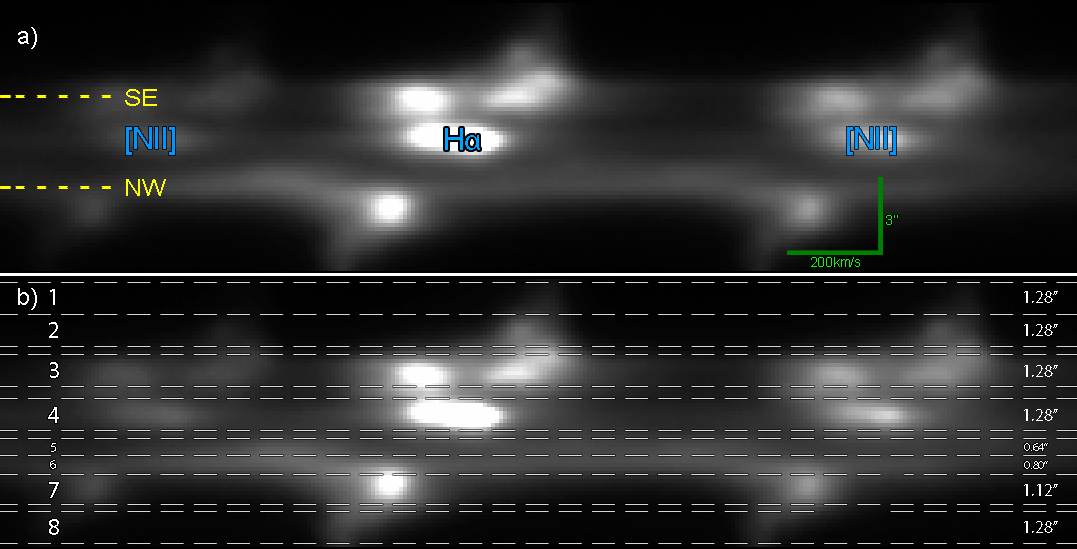
\includegraphics[width=\linewidth]{figures/xshooter_ic5063/apertures.png}
	\caption[Two-dimensional long-slit spectra along the radio axis of IC\;5063, with the positions of extracted apertures overlaid.]{\textbf{a)}: Two-dimensional spectrum of the H$\mathrm{\alpha}$+[NII] emission lines at $\sim$6560\;{\AA} in the VIS arm of the Xshooter data of IC\;5063, showing the line profiles in the inner regions of the galaxy. The spectral axis is horizontal and the spatial axis is vertical; the velocity and spatial scales are shown as a labelled green axis. The centroids of the radio lobes --- measured from 24.8\;GHz radio continuum imaging presented by \citet{Morganti2007} --- are shown as yellow dashed lines, and each lobe is labelled. \textbf{b)}: The same as in a), but with apertures selected for the UVB and VIS arms marked with white dashed lines and labelled as `1-8' on the left; the spatial width of each aperture in arcseconds is given on the right. Note that the H$\mathrm{\alpha}$+[NII] blend is shown here for presentation purposes, as it clearly demonstrates the emission-line structure of forbidden ([NII]) and permitted (H$\alpha$) species.}
	\label{fig: xshooter_ic5063: apertures}
\end{figure*}

Finally, the extracted and corrected UVB and VIS one-dimensional spectra were combined to produce a single one-dimensional spectrum for each aperture, covering the full wavelength range of both arms. During this process, the spectra for both arms were resampled to a common wavelength grid with steps of $\Delta\lambda$ = 1{\;\AA} using the \textsc{SpectRes} \citep{Carnall2017}, \textsc{specutils} \citep{Earl2021} and \textsc{Astropy} \citep{AstropyCollaboration2013, AstropyCollaboration2018} \textsc{Python} packages. $\Delta\lambda = 1${\;\AA} was chosen for the resampling because this was the smallest wavelength step allowed by the base stellar templates used in the stellar continuum modelling (described in Section\;\ref{section: xshooter_ic_5063: observations_and_data_reduction: starlight}). 

Because of the different spatial pixel scale of Xshooter's NIR arm relative to its UVB and VIS arms, the NIR data was considered separately. Apertures for the NIR data were derived from the UVB+VIS apertures by first fitting two Gaussian profiles to a spatial slice of the continuum near the [OIII]$\lambda\lambda$5007,4959 doublet and taking the centroid of the narrowest to be the position of the continuum peak along the slit --- the distances from the centre of each UVB+VIS aperture to this continuum peak were then calculated. The same procedure was used to identify the continuum peak in the NIR arm using a continuum slice adjacent to the near-infrared HeI$\lambda$10830 line. The ratio of the VIS+UVB pixel scale (0.16\;arcsec/pixel) to the NIR pixel scale (0.21\;arcsec/pixel) was then used to convert the aperture distances and widths from the UVB+VIS arm to the NIR arm. It should be noted that the spatial boundaries of the NIR apertures are not exactly the same as the UVB+VIS apertures due to the different pixel scales of the arms, the fact that the apertures are only a few pixels wide, uncertainties related to the Gaussian fits to the continuum spatial slices, and the fact that aperture spatial positions are only measured to an accuracy of 0.1\;pixels.

\subsection{Stellar continua modelling and subtraction}
\label{section: xshooter_ic_5063: observations_and_data_reduction: starlight}

Following the selection, extraction, and correction of the UVB+VIS apertures, the underlying stellar continua in each were modelled and subtracted using the \textsc{STARLIGHT} stellar spectral synthesis code (version 4: \citealt{CidFernandes2005, Mateus2006}), making use of the \textsc{STELIB} empirical stellar templates \citep{LeBorgne2003} and the stellar population synthesis model presented by \citet{Bruzual2003}. This was done to ensure that measured emission-line fluxes used in the analysis were as accurate as possible and did not suffer from the effects of underlying stellar absorption.

In order to ensure good fits to the stellar continua, any spectral features not associated with a stellar component (such as AGN emission lines and any residual telluric absorption) were excluded from the fitting process. The normalising region for the fits was chosen to be 4740--4780{\;\AA}; the total wavelength range covered in the \textsc{STARLIGHT} fits was 3220--8000{\;\AA}. The adequacy of the resulting fits was checked visually by closely inspecting key absorption features that do not suffer from emission-line contamination, such as the MgI absorption feature at 5167\;{\AA} (Figure\;\ref{fig: xshooter_ic5063: starlight_mgi_ni}) and the CaII K absorption feature at 3934\;{\AA} (Figure\;\ref{fig: xshooter_ic5063: starlight_caii_hk_heta}), as well as the fit to the overall continuum shape. After being deemed acceptable, the modelled stellar flux densities were subtracted from the observed flux densities in each aperture. 

To further highlight the necessity of proper continuum subtraction, in Figure\;\ref{fig: xshooter_ic5063: starlight_hgamma_oiii} I present the stellar continuum fits in the region of the H$\mathrm{\gamma}$ and [OIII]$\lambda$4363 emission lines, and in Figure\;\ref{fig: xshooter_ic5063: starlight_heii_ariv} I present the stellar continuum fits in the region of the HeII and [ArIV]$\lambda\lambda4711,4740$ emission lines.

\begin{figure*}
    \begin{subfigure}[t]{0.47\textwidth}
        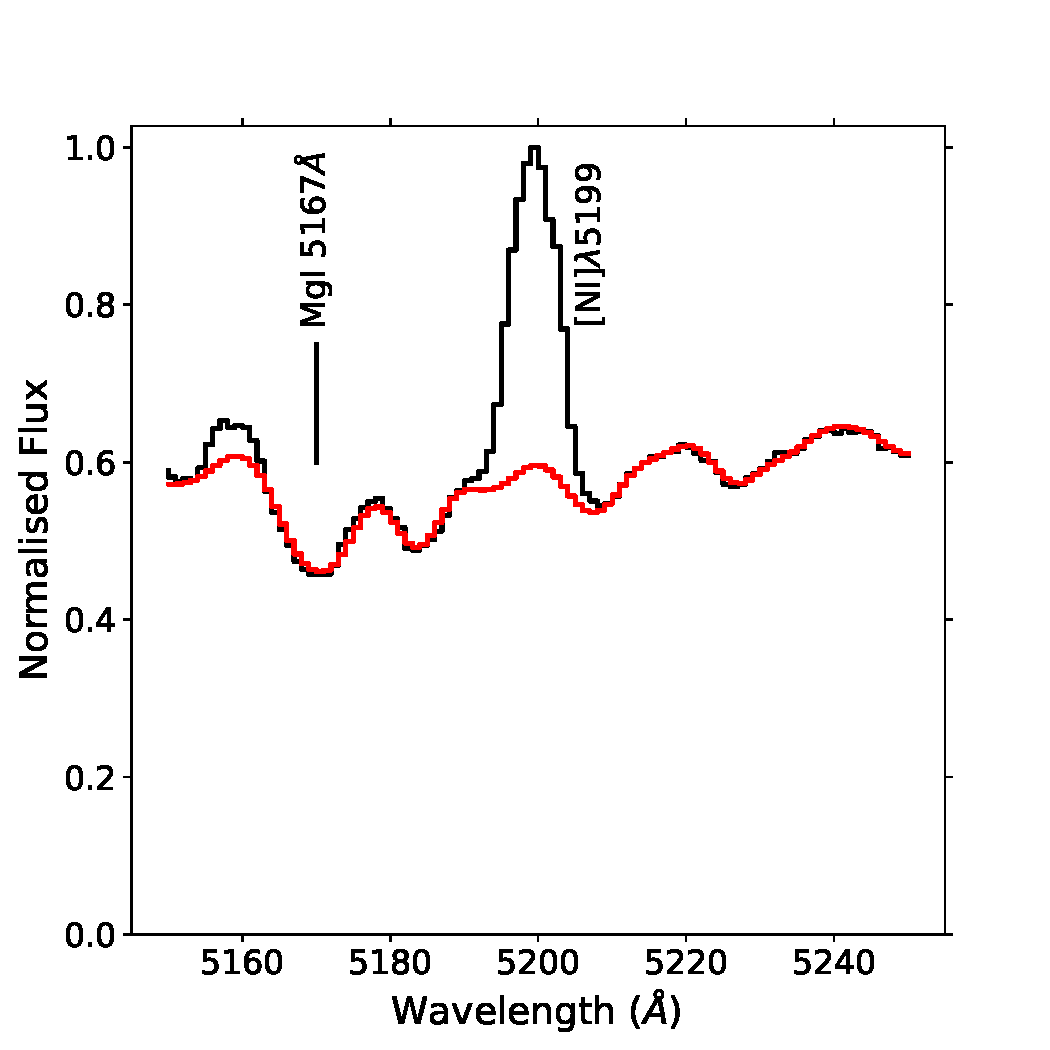
\includegraphics[width=\linewidth]{figures/xshooter_ic5063/starlight_mgi_ni.pdf}
        \caption{The spectral region of the MgI 5167\;{\AA} absorption feature and the [NI]$\lambda$5199 emission line.}
        \label{fig: xshooter_ic5063: starlight_mgi_ni}
    \end{subfigure}
    \hfill
    \begin{subfigure}[t]{0.47\textwidth}
        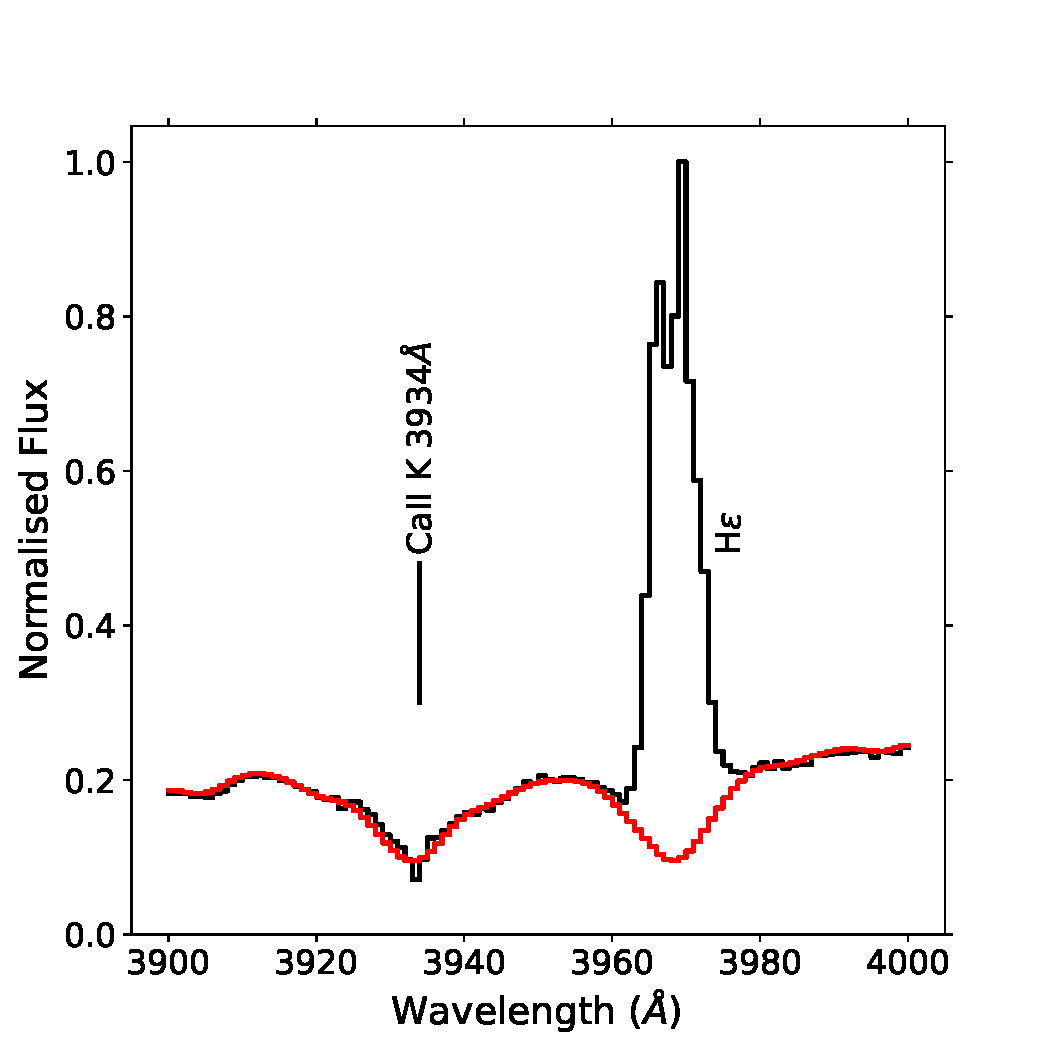
\includegraphics[width=\linewidth]{figures/xshooter_ic5063/starlight_caii_hk_hep.pdf}
        \caption{The spectral region of the CaII K absorption feature at 3934\;{\AA}, and the H$\mathrm{\varepsilon}$ recombination line.}
        \label{fig: xshooter_ic5063: starlight_caii_hk_heta}
    \end{subfigure}
    \vspace{2cm}
    \begin{subfigure}[t]{0.47\textwidth}
        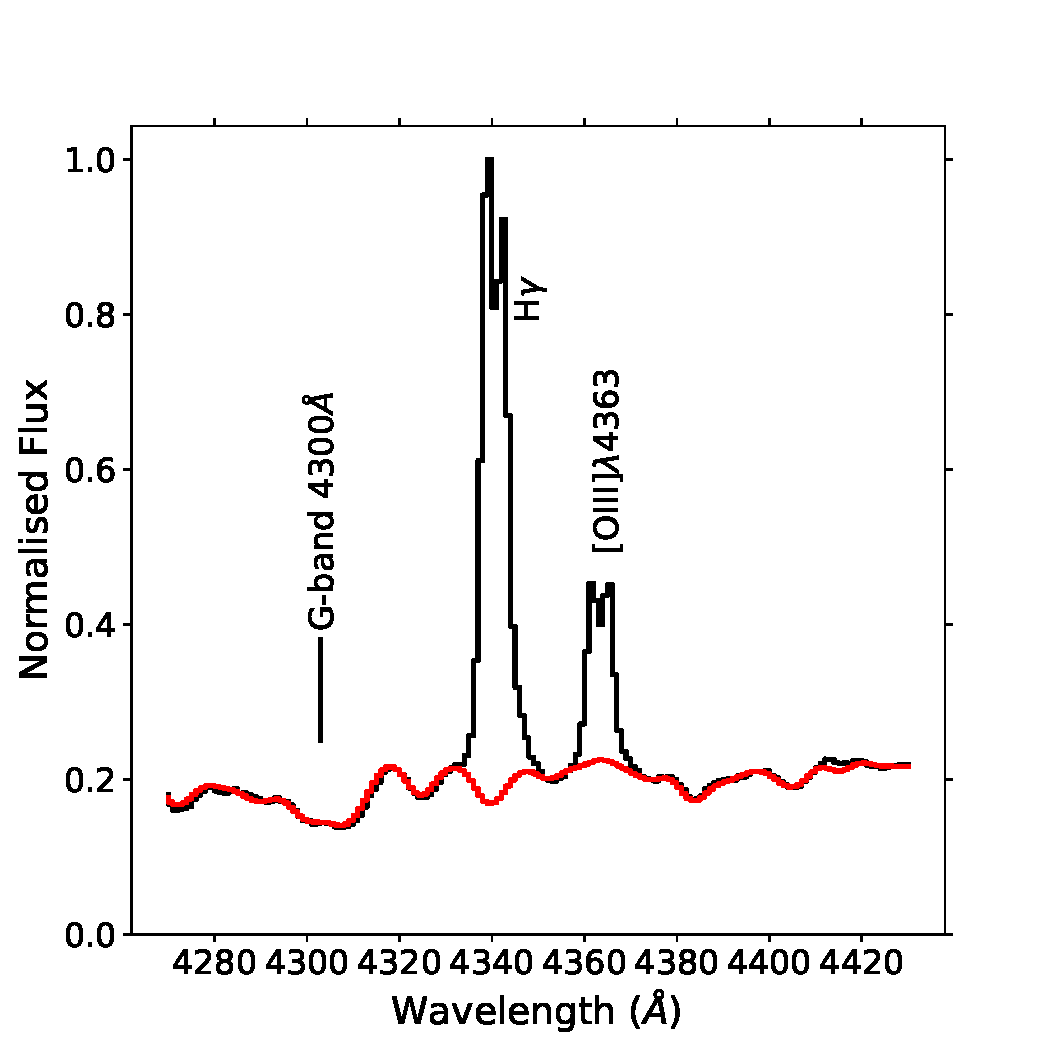
\includegraphics[width=\linewidth]{figures/xshooter_ic5063/starlight_hgamma_oiii4363.pdf}
        \caption{The spectral region of the H$\mathrm{\gamma}$ and [OIII]$\lambda$4363 emission lines; the fit to the G-band stellar absorption feature at $\sim$4300\;{\AA} can also be seen.}
        \label{fig: xshooter_ic5063: starlight_hgamma_oiii}
    \end{subfigure}
    \hfill
    \begin{subfigure}[t]{0.47\textwidth}
        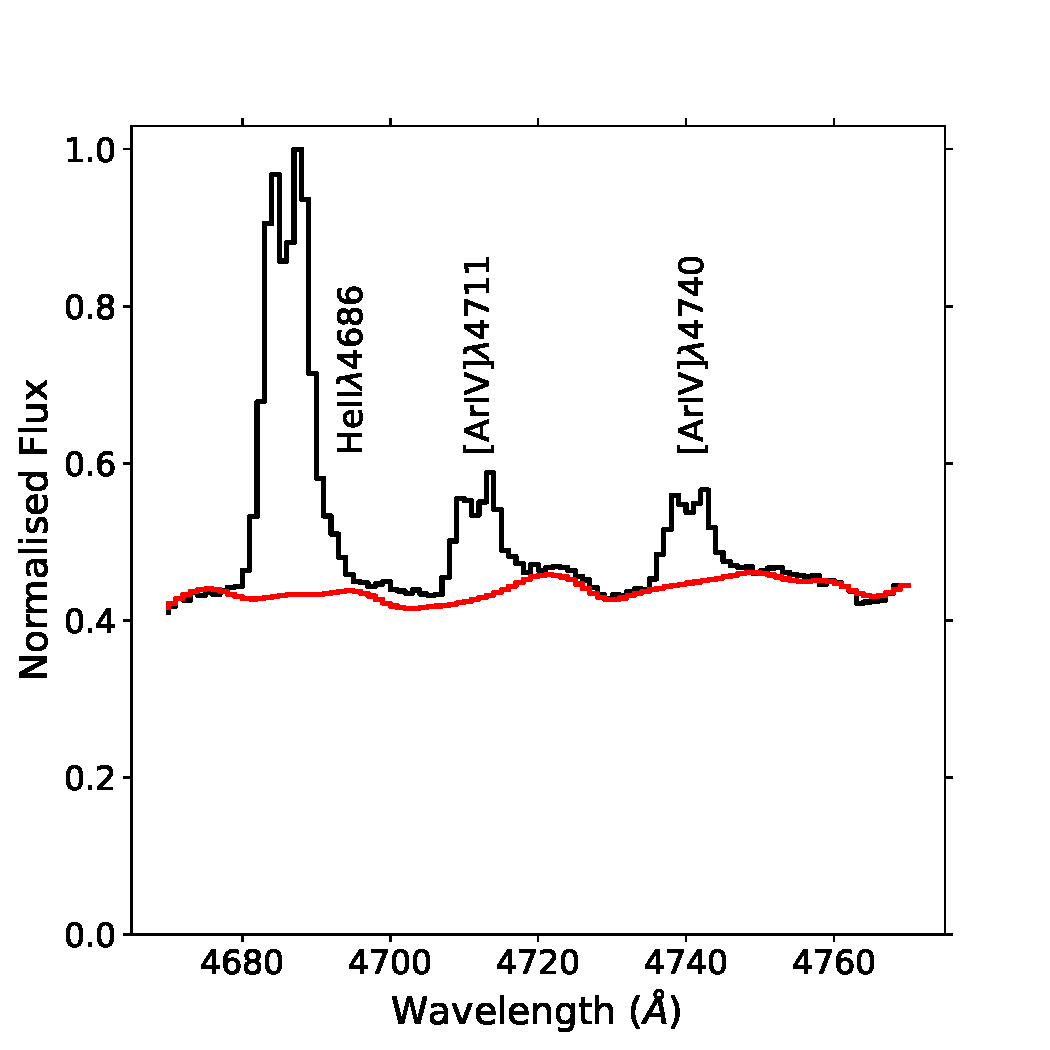
\includegraphics[width=\linewidth]{figures/xshooter_ic5063/starlight_ariv.pdf}
        \caption{The spectral region of the HeII$\lambda$4686 and [ArIV]$\lambda\lambda$4711,4740 emission lines.}
        \label{fig: xshooter_ic5063: starlight_heii_ariv}
    \end{subfigure}
    \vspace{-1.5cm}
    \caption[\textsc{STARLIGHT} stellar-synthesis fits to various key spectral features in Xshooter spectra of IC\;5063.]{\textsc{STARLIGHT} fits (red solid line) to various features in the spectrum extracted from Aperture 3 of the Xshooter UVB+VIS data (solid black line); the emission and absorption lines shown in each plot are labelled. Complex stellar continuum structure, which may significantly affect the derived line fluxes, can be seen underneath emission lines in several cases, and contributes significantly to the profiles of the [ArIV] lines. Therefore, proper modelling and subtraction was necessary to ensure accurate measurements of line fluxes.}
\end{figure*}

\subsection{Emission-line fitting}
\label{section: xshooter_ic_5063: observations_and_data_reduction: emission_line_fitting}

After stellar-continuum subtraction, the profiles of key emission lines in each aperture were fit with Gaussian profiles and a low-order-polynomial (to account for non-stellar continua in the UVB+VIS arms, and overall continuum structure in the NIR arm) using \textsc{Python} scripts written with the \textsc{NumPy} \citep{Harris2020}, \textsc{Pandas} \citep{reback2020pandas}, \textsc{AstroPy}, and \textsc{specutils} packages. In all cases, several Gaussian components were required to properly fit the emission-line profiles, however, to prevent overfitting, it was important to only use as few Gaussians as possible while still producing an adequate fit to the line profiles. Therefore, further Gaussian components were only added if they significantly reduced the mean-square residuals and $\chi^2$ of the fit. Furthermore, a sum-of-squares f-test \citep{Montgomery2012} was used to ensure that the relative decrease in residuals with each added Gaussian component was statistically significant (at the $\alpha=0.01$ significance level). This took into account the degrees of freedom of the total model when adding additional Gaussian components, preventing overfitting.

Emission-line-profile models for the combined UVB+VIS data were produced by first fitting the [OIII]$\lambda\lambda$4959,5007 doublet. Gaussian components were simultaneously fitted to both lines in the doublet, with each pair of Gaussian components having the same FWHM, and a wavelength separation (49.9\;{\AA}) and intensity ratio ($1:2.99$) defined by atomic physics \citep{Osterbrock2006}. The resulting multiple-Gaussian-component fits to the [OIII]$\lambda\lambda$4959,5007 doublet are hereafter referred to as the `[OIII] models'; these are shown for each aperture in Figure\;\ref{fig: xshooter_ic5063: o3_models}. For each aperture, narrow (FWHM$_\mathrm{w}$\;\textless\;200\;km\;s$^{-1}$: see Section\;\ref{section: xshooter_ic5063: properties_of_outflowing_gas: uvb_vis_analysis_and_results: kinematics}) and broad (FWHM$_\mathrm{w}$\;\textgreater\;500\;km\;s$^{-1}$) components of the [OIII] line profiles were identified. The former have kinematics consistent with gravitational (rotational) motions in the host galaxy (as deduced from large-scale HI\;21\;cm and CO kinematics: \citealt{Morganti1998, Morganti2015}), and the latter are consistent with outflowing gas. The broad components have complex, often multi-peaked profiles that required fitting with a combination of Gaussian components of different widths. Note that the \textit{individual} Gaussian components used to fit the broad components are not interpreted as physically-distinct kinematic components --- rather, they are required to account for the \textit{total} flux in the broad part of the line profiles.

Whereas in most apertures the [OIII] profiles can be well-described by one total broad and one total narrow component (each modelled with more than one Gaussian component), Aperture\;3 is an exception to this because there are two clearly separated `narrow' components and a single broad component in the [OIII]$\lambda\lambda$4959,5007 line profiles. In this case, the two narrow components are considered separately, and are labelled `Narrow 1' (red-most) and `Narrow 2' (blue-most). In apertures 4 and 5, the majority of the components are broad and heavily blended, and therefore only the total line fluxes (narrow + broad) are considered.

The [OIII] models were used to constrain the fits to the other UVB+VIS emission lines used in this analysis, namely H$\mathrm{\beta}$, H$\mathrm{\gamma}$, [OIII]$\lambda$4363, [OII]$\lambda$3726,3729, [OII]$\lambda\lambda$7319,7331, [SII]$\lambda\lambda$4068,4076, [SII]$\lambda\lambda$6717,6731, [ArIV]$\lambda\lambda$4711,4740 and HeII$\lambda$4686 --- the fits to these lines for Aperture 3 are shown in Figure\;\ref{fig: xshooter_ic5063: o3_models_all_lines}. I note that fits for H$\mathrm{\alpha}$ and the [NII]$\lambda\lambda$6548,6583 doublet were not produced for apertures with complex, broad emission-line profiles, as the lines were significantly blended and thus it was not possible to precisely measure their fluxes due to degeneracy issues. For all fits to the other lines, the intensity of each Gaussian component was allowed to vary, while the wavelength separations\footnote{When fitting the [OIII] models to other lines, the centroid wavelength of the brightest narrow component was allowed to vary by $\pm$1{\;\AA} in order to provide a better fit within the limit of the $\Delta\lambda$ = 1{\;\AA} resampling.} and widths of the Gaussian components were fixed. For some of the weaker emission lines with much lower fluxes than the [OIII]$\lambda\lambda$4959,5007 doublet, the fainter Gaussian components were sometimes excluded from the fits since the line-profile features they accounted for were extremely faint relative to the continuum.

For the emission lines that were fitted, including the transauroral [SII]$\lambda\lambda$4068,4076 and [OII]$\lambda\lambda$7319,7331 doublets, it was found that the [OIII] models describe their profiles well in all cases. In contrast, it was found that the [OIII] models do not describe emission lines in the NIR arm well, such as [FeII]$\lambda$12570, [FeII]$\lambda$16400, H$_2 \lambda$21218, Pa$\beta$, Br$\gamma$ and HeI$\lambda$10830. This is likely a result of the lack of stellar continua subtraction for the NIR data, which is due to the limited wavelength range of the \textsc{STARLIGHT} fits (3220--8000\;\AA), the lower cosmetic quality of the NIR spectra, and the difficulty in exactly matching the NIR apertures to the UVB+VIS apertures spatially. Therefore, each line in the NIR arm was fitted independently. \\

\begin{figure*}
	\includegraphics[width=\linewidth, trim={0cm 0cm 1cm 0cm},clip]{figures/xshooter_ic5063/oiii_models.png}
	\caption[{[}OIII{]} line profile models for the apertures extracted along the radio axis of Xshooter spectra of IC\;5063.]{[OIII]$\lambda\lambda$4959,5007 rest-frame line profiles and models for the apertures covering the inner regions of IC\;5063. The observed line profiles are shown in black, the overall fits to the profiles are shown as red solid lines, the Gaussian components comprising the total narrow component are shown as blue dashed lines, and the Gaussian components comprising the total broad component are shown as dotted green lines. Fitting residuals are shown as black dots below each line profile. In the cases of apertures 4 and 5, each Gaussian component is shown as a purple dash-dotted line, as there is no distinction made between broad and narrow. The wavelengths corresponding to the percentile ($v_\mathrm{p}$; $v_\mathrm{05}$ and $v_\mathrm{95}$) and the flux-weighted velocities ($v_\mathrm{w}$) for Aperture 5 are shown as dashed grey lines. For Aperture 6, dashed grey lines mark the wavelengths of the percentile velocity of the broad component ($v_\mathrm{p,b}$) and flux-weighted velocity of the narrow component ($v_\mathrm{w,n}$) --- these are used to calculate the outflow velocity ($v_\mathrm{out}$ = $v_\mathrm{p,b}$ - $v_\mathrm{w,n}$). Aperture 3 presents two clearly split narrow components, which are labelled `Narrow 1' (red-most) and `Narrow 2' (blue-most).}
	\label{fig: xshooter_ic5063: o3_models}
\end{figure*}

\begin{figure*}
	\includegraphics[width=\linewidth]{figures/xshooter_ic5063/oiii_fits_other_lines.png}
	\caption[{[}OIII{]}-model fits to key emission lines used in the analysis of Xshooter observations of IC\;5063.]{Fits to key diagnostic emission lines in Aperture 3 of the UVB+VIS spectra using the [OIII] model for Aperture 3 (shown in Figure\;\ref{fig: xshooter_ic5063: o3_models}). Where lines from multiple atoms are present, they are labelled by both atom and species. The diagnostic lines shown here are used in this chapter to derive key outflow properties.}
	\label{fig: xshooter_ic5063: o3_models_all_lines}
\end{figure*}

\newpage

\section{Properties of the outflowing gas}
\label{section: xshooter_ic5063: properties_of_outflowing_gas}

\subsection{Analysis of the UVB+VIS apertures}
\label{section: xshooter_ic5063: properties_of_outflowing_gas: uvb_vis_analysis_and_results}

\subsubsection{Velocity shifts and widths}
\label{section: xshooter_ic5063: properties_of_outflowing_gas: uvb_vis_analysis_and_results: kinematics}

The Doppler shifts and widths of broad and narrow components of the [OIII] models, relative to the lab wavelength\footnote{Note that the Xshooter spectra were de-redshifted, as described in Section\;\ref{section: xshooter_ic_5063: observations_and_data_reduction: data_reduction}.} of [OIII]$\lambda$5007, were used to determine outflowing and quiescent (non-outflowing) gas kinematics. First, the instrumental broadening (as measured from the Galactic NaID lines) was subtracted from the width of each component in quadrature in order to produce the intrinsic line widths.

When deriving outflow kinematics, projection effects must be carefully considered (see Section\;\ref{section: introduction: outflows: kinematics_and_geometry: kinematics}). Therefore, two methods for estimating outflow velocity were used, giving `minimal' and `maximal' velocities, following the methodology presented by \citet{Rose2018}. The first approach was to calculate flux-weighted mean velocity shifts and widths --- this was done for the total broad and narrow components by weighting the centroid velocities and FWHM of each constituent Gaussian component by its total flux:

\begin{equation}
v_\mathrm{w} = \frac{\Sigma_i(F_i \times v_i)}{\Sigma_i{F_i}}\text{, and}
\label{eq: xshooter_ic5063: flux_velocity}
\end{equation}

\begin{equation}
\mathrm{FWHM_w} = \frac{\Sigma_i(F_i{\times}\mathrm{FWHM_i})}{\Sigma_i{F_i}},
\label{eq: xshooter_ic5063: flux_width}
\end{equation}
\noindent
where $F_\mathrm{i}$, FWHM$_\mathrm{i}$ and $v_\mathrm{i}$ are the fluxes, FWHMs and velocity shifts of the constituent Gaussian components, respectively. Velocity shifts were calculated using the wavelength shifts of a given centroid to the lab wavelength of [OIII]$\lambda$5007; for the broad components, this is likely to underestimate true outflow velocities.

Percentile velocities were also derived by using the far wings of the broad-component profiles, as described in Section\;\ref{section: introduction: outflows: kinematics_and_geometry: kinematics}. Here, it is assumed that all line broadening is due to different projections of velocity vectors along the line of sight, rather than intrinsic velocity dispersion in the gas in each volume element. In this case, the extended velocity wings represent gas moving directly along the line of sight, and potentially give a better estimate of the true outflow velocity. Therefore, velocity widths are not reported in this case. Percentile velocity shifts were determined for the broad components using the wavelength which contains either 5 or 95 per cent of the total flux of the line profile relative to the lab wavelength of [OIII]$\lambda$5007 (whichever velocity was greater, to ensure that outflow kinematics were not underestimated). Velocities derived in this way are labelled $v_\mathrm{p}$. As an example, in Figure\;\ref{fig: xshooter_ic5063: o3_models} both the percentile ($v_\mathrm{p}$) and flux-weighted ($v_\mathrm{w}$) velocity for the [OIII] profile of Aperture 5 are shown.

\begin{table*}
	\renewcommand{\arraystretch}{1}
	\begin{tabular}{lcccccc}
	\multirow{2}{*}{Component} & Distance   & Distance  & $v_\mathrm{p}$  & $v_\mathrm{w}$  & FWHM$_\mathrm{w}$     & $v_\mathrm{out}$  \\ 
        & (arcsec) & (kpc) & (km\;s$^{-1}$) & (km\;s$^{-1}$) & (km\;s$^{-1}$) & (km\;s$^{-1}$) \\
        \\
    \hline \\
	AP1 Narrow       & $-$4.72             & $-$1.09          & ---    & 218$\pm$5    & 120$\pm$3  &                  \\
		&	&	&	&	&	&	\\
	AP2 Narrow       & $-$3.44             & $-$0.79          & ---    & 197$\pm$3    & 110$\pm$2  &                  \\
		&	&	&	&	&	&	\\
	AP3 Narrow 1     & $-$1.84             & $-$0.43          & ---    & 166$\pm$3    & 158$\pm$4  &                  \\
	AP3 Narrow 2     & $-$1.84             & $-$0.43          & $-$202$\pm$2   & $-$68$\pm$1    & 187$\pm$3  & $-$233$\pm$4$^a$   \\
	AP3 Broad        & $-$1.84            & $-$0.43          & 507$\pm$23   & 121$\pm$8    & 549$\pm$36 & 341$\pm$23   \\ 
		&	&	&	&	&	&	\\
	AP4 Total        & 0                 & 0              & 264$\pm$41   & $-$7$\pm$2     & 296$\pm$16 &                  \\
		&	&	&	&	&	&	\\
	AP5 Total        & 1.36              & 0.31           & $-$699$\pm$173 & $-$102$\pm$8   & 670$\pm$27 & $-$699$\pm$173$^b$ \\
		&	&	&	&	&	&	\\
	AP6 Narrow       & 2.08              & 0.48           & ---   & $-$193$\pm$4   & 102$\pm$4  &                  \\
	AP6 Broad        & 2.08              & 0.48           & $-$714$\pm$156 & $-$198$\pm$15  & 614$\pm$58 & $-$521$\pm$156 \\
		&	&	&	&	&	&	\\
	AP7 Narrow       & 3.04              & 0.70           & ---  & $-$166$\pm$4   & 163$\pm$4  &                  \\
	AP7 Broad        & 3.04              & 0.70           & $-$624$\pm$85  & $-$166$\pm$13  & 627$\pm$57 & $-$457$\pm$85   \\ 
		&	&	&	&	&	&	\\
	AP8 Narrow       & 4.48              & 1.03           & ---  & $-$197$\pm$17 & 157$\pm$18 &                  \\
		&	&	&	&	&	&	\\
	\end{tabular} \\
	$^a$ calculated using the flux-weighted velocities ($v_\mathrm{w}$) for AP3 Narrow 1 (quiescent gas) and AP3 Narrow 2 (in/out-flowing gas). \\
	$^b$ the same as the percentile velocity ($v_\mathrm{p}$) since there is no corresponding narrow component.\\
	\caption[Warm-ionised gas kinematics along the radio structure of IC\;5063.]{The kinematics for the broad and narrow components in each aperture, including the percentile velocities ($v_\mathrm{p}$; the velocity that contains 5 or 95\;per\;cent of the flux of the emission-line profile), flux-weighted velocities ($v_\mathrm{w}$; determining used flux-weighted velocity averages), and corresponding flux-weighted velocity widths (FWHM$_\mathrm{w}$). The outflow velocity ($v_\mathrm{out}$) is taken to be the difference between the percentile velocity of the outflowing broad components and the flux-weighted velocity of the quiescent narrow components at each position. The distances from the centre of Aperture 4 (the nucleus) to the centre of the aperture for each component are also given in both arcseconds and kpc. For Aperture 3, `Narrow 1' and `Narrow 2' denote the two narrow components of the split line profile (see Figure\;\ref{fig: xshooter_ic5063: o3_models}), with `Narrow 2' being the blue-most narrow component}
	\label{tab: xshooter_ic5063: kinematics}
\end{table*}

\begin{figure*}
    \centering
	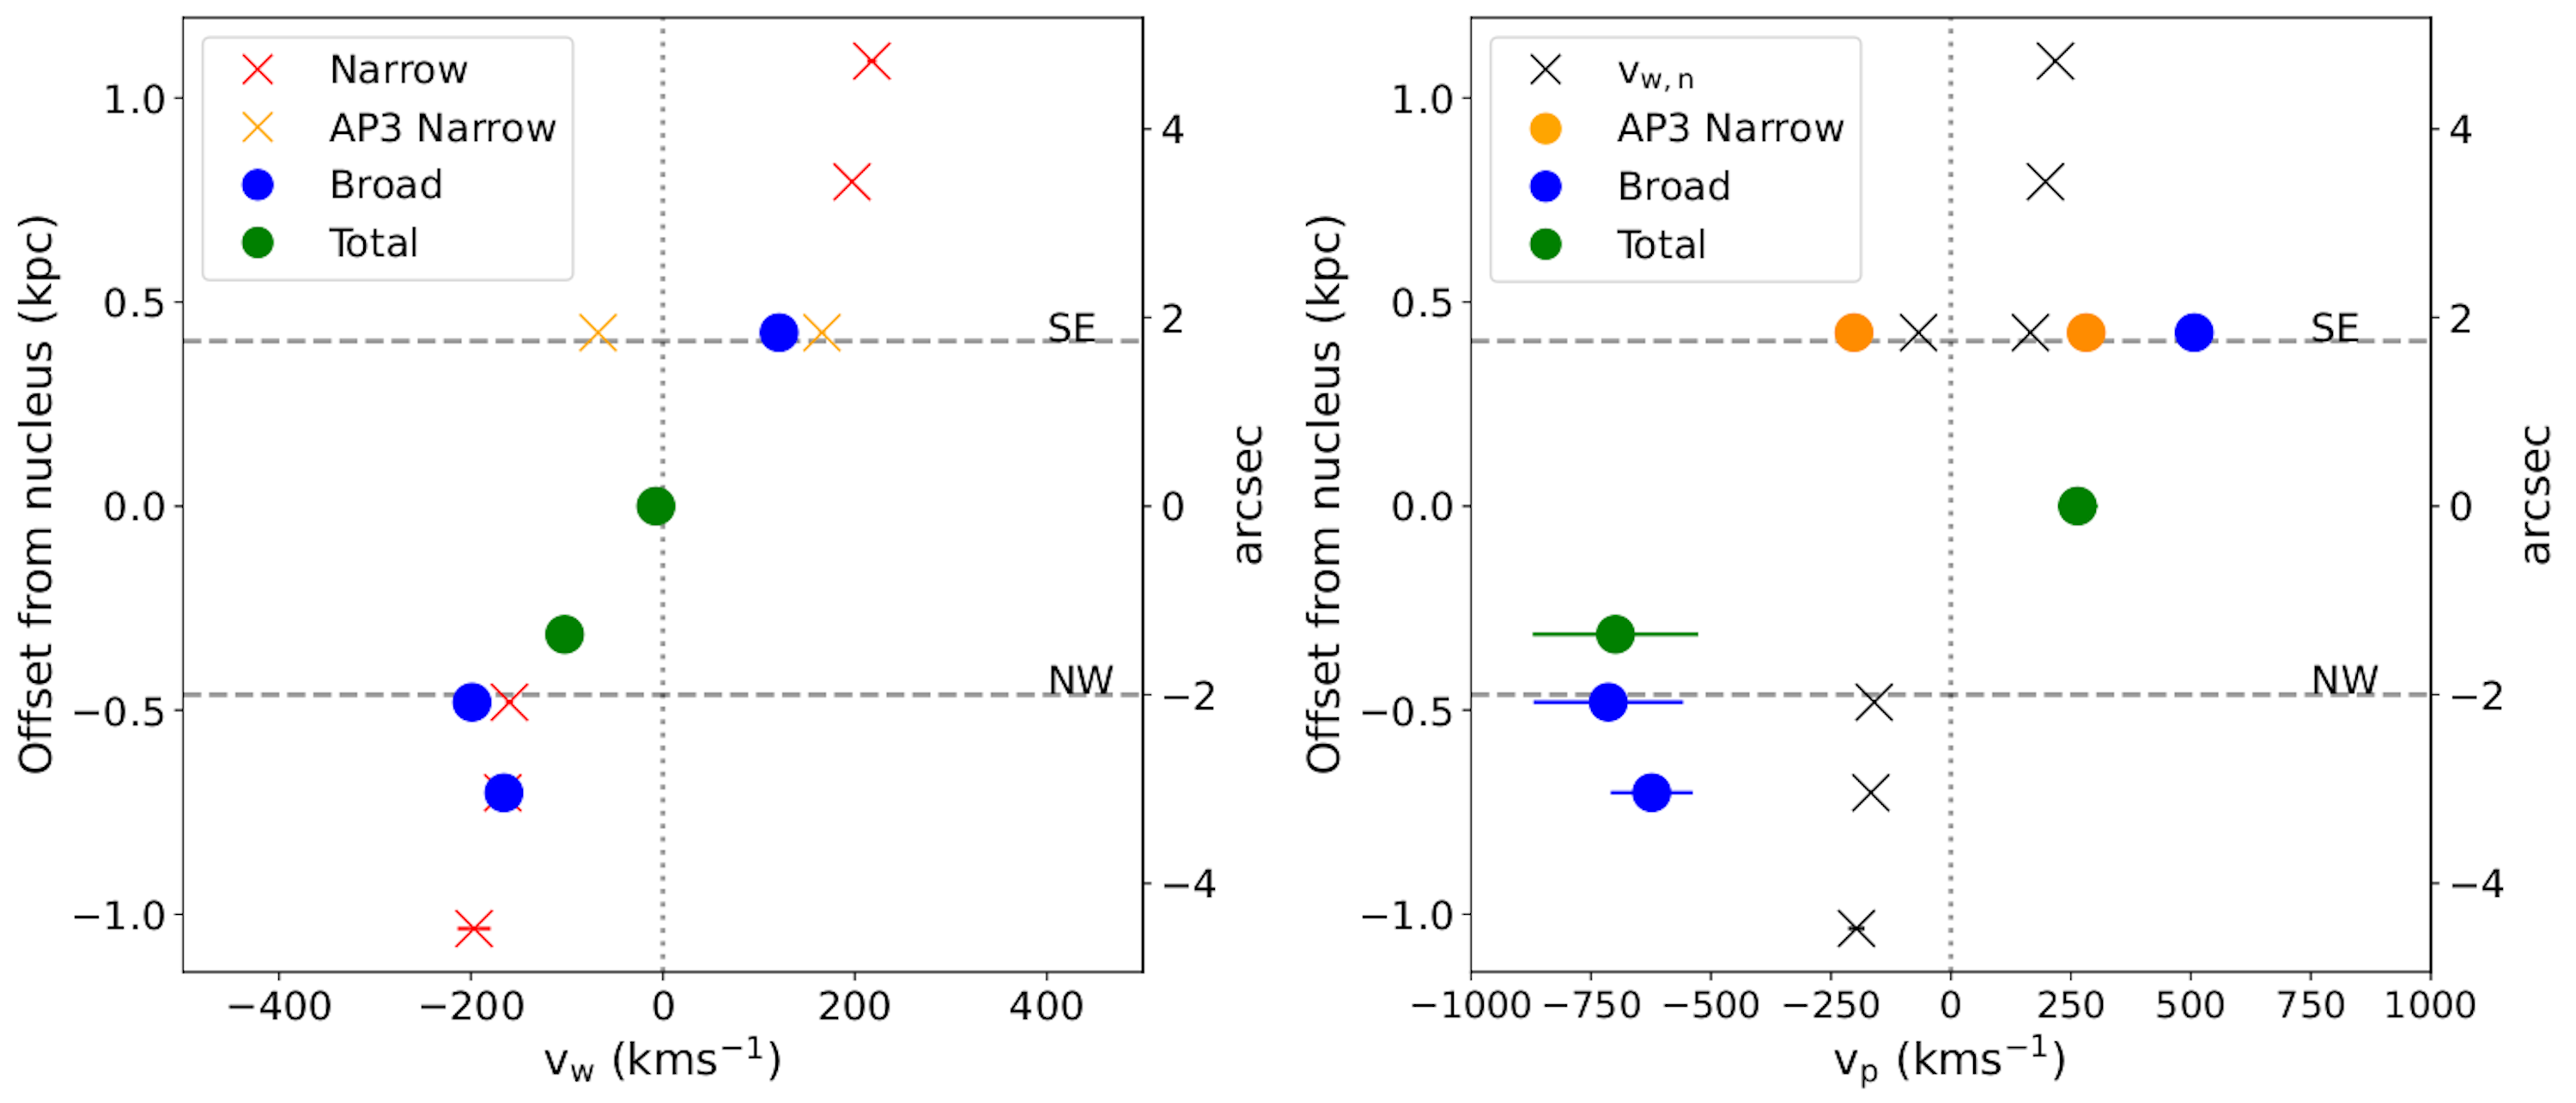
\includegraphics[width=\linewidth]{figures/xshooter_ic5063/vmin_vmax.png}
	\caption[Velocity shifts of the warm-ionised gas along the radio structure of IC\;5063.]{Velocity shifts for narrow (red crosses), broad (blue circles), and total (green circles) kinematic components in each aperture, shown spatially across the radio structure of IC\;5063. The split narrow components in Aperture 3 are shown in orange. The spatial position of each component corresponds to the centre of the aperture in which it was measured. \textbf{Left}: flux-weighted velocities of the narrow and broad components --- the narrow components are taken to represent the galaxy's quiescent rotating gas disk. \textbf{Right}: percentile velocity shifts ($v_\mathrm{p}$) for the broad components, taken to represent outflowing gas, compared with the flux-weighted velocities of the narrow components ($v_\mathrm{w,n}$, shown for reference as black crosses). The dashed grey lines mark the centroids of the NW and SE radio lobes, measured from 24.8\;GHz continuum imaging presented by \citet{Morganti2007}. A velocity shift of zero relative to the galaxy's rest frame is marked with a grey dotted line.}
	\label{fig: xshooter_ic5063: velocities}
\end{figure*}

\begin{figure}
    \centering
	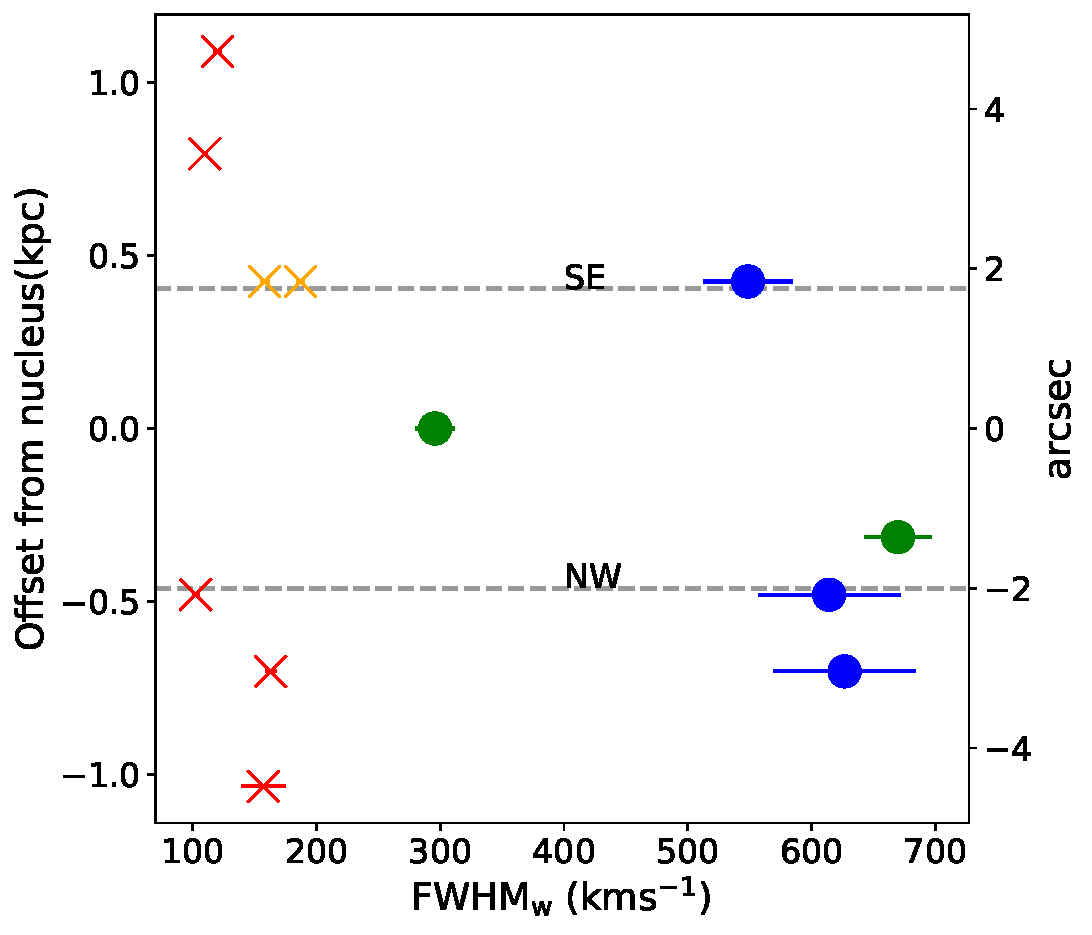
\includegraphics[width=0.55\linewidth]{figures/xshooter_ic5063/vmin_widths.pdf}
	\caption[Velocity widths of the warm-ionised gas along the radio structure of IC\;5063.]{Flux-weighted velocity widths (FWHM$_\mathrm{w}$) as determined in the minimal velocity case, in which the measured velocity widths are assumed to be entirely due to local velocity dispersion within the outflow. The colour and marker scheme and dashed lines are the same as in Figure\;\ref{fig: xshooter_ic5063: velocities}.}
	\label{fig: xshooter_ic5063: fwhm}
\end{figure}

\newpage
Figure\;\ref{fig: xshooter_ic5063: velocities} shows a position-velocity (PV) diagram of the percentile ($v_\mathrm{p}$) and flux-weighted ($v_\mathrm{w}$) velocity shifts, as measured in each aperture, and Figure\;\ref{fig: xshooter_ic5063: fwhm} shows the flux-weighted velocity widths. In the flux-weighted case ($v_\mathrm{w}$; right panel of Figure\;\ref{fig: xshooter_ic5063: velocities}), the velocity shifts of the narrow components (with the exception of the blue-most narrow component in Aperture 3) appear to follow a rotation curve of amplitude $\pm$218\;km\;s$^{-1}$, corresponding to the rotational motion of the galaxy's disk (as seen in HI\;21\;cm and CO observations: \citealt{Morganti1998, Morganti2015, Oosterloo2017}). Deviations from this rotation curve can be seen in the percentile velocity shifts of the broad components and the total line profile in Aperture 5 (which is dominated by broad components), indicating that the broad components represent outflowing gas. Interestingly, this deviation is not seen in the flux-weighted case, indicating that the outflows are kinematically symmetric relative to the disk rotation. 

One of the narrow components observed in the line profile of Aperture 3 (`AP3 Narrow 2') shows significant deviation ($v\sim350$\;km\;s$^{-1}$) from the rotation curve, indicating that it is a distinct kinematic component which may represent outflowing or inflowing gas. 

From these kinematics, the broad components in apertures 3, 6 and 7, along with the `AP3 Narrow 2' component and the total line profile of Aperture 5, are taken to represent outflowing gas. Note that the broad components in apertures 1, 2 and 8 are most likely due to spill-over from the broad profiles in the central apertures due to the beam-smearing effect of atmospheric seeing --- not locally outflowing gas --- and as such are not considered to represent outflows at these locations. Since the kinematics of the narrow components are consistent with quiescent gas in a rotating disk, the outflow velocity in each aperture was thus taken to be the difference between the percentile velocity ($v_\mathrm{p}$) of the broad component (outflow) and the flux-weighted velocity ($v_\mathrm{w}$) of the narrow component (quiescent) --- an example of this for Aperture 6 is shown in Figure\;\ref{fig: xshooter_ic5063: o3_models}. For Aperture 5, where the majority of the components are broad and the narrow components (representing emission from the rotating disk) are heavily blended, the outflow velocity is taken to be the percentile velocity. The derived flux-weighted, percentile, and outflow velocities (in addition to the velocity widths) are given in Table\;\ref{tab: xshooter_ic5063: kinematics}.

\subsubsection{Spatial distributions and kinematics of optical diagnostic lines}
\label{section: xshooter_ic5063: properties_of_outflowing_gas: uvb_vis_analysis_and_results: spatial_distributions}

\begin{table}
    \vspace*{1cm}
	\centering
	\renewcommand{\arraystretch}{1.5}
	\begin{tabular}{ccc}
	Emission Line           &  Centroid (pixels) & Centroid (arcsec) \\ \hline
	[OIII]$\lambda$5007 & 12.3$\pm$0.1                                                                                                       & 1.97$\pm$0.02                                                                                                             \\
	H$\beta$                & 12.5$\pm$0.1                                                                                                       & 2.00$\pm$0.02                                                                                                             \\
	{[}OII{]}$\lambda$7319  & 11.9$\pm$0.1                                                                                                       & 1.90$\pm$0.02                                                                                                             \\
	{[}SII{]}$\lambda$4069  & 12.0$\pm$0.1                                                                                                       & 1.92$\pm$0.02                                                                                                            
	\end{tabular} \\
	\caption[The spatial positions of the peak flux of the blue wings of the transauroral {[}OII{]} and {[}SII{]} lines, in addition to {[}OIII{]}$\lambda5007$ and H$\beta$ lines]{Centroids of Gaussian fits to spatial slices between \mbox{$-$600\;\textless\;$v$\;\textless\;$-$400\;km\;s$^{-1}$} of the transauroral [OII] and [SII] emission lines, along with H$\mathrm{\beta}$ and [OIII]$\lambda$5007 (shown in Figure\;\ref{fig: xshooter_ic5063: spatial_optical}), relative to the spatial position of the continuum centre.}
	\label{tab: xshooter_ic5063: spatial_vis}
\end{table}

\begin{figure}[!ht]
    \vspace*{1cm}
	\centering
	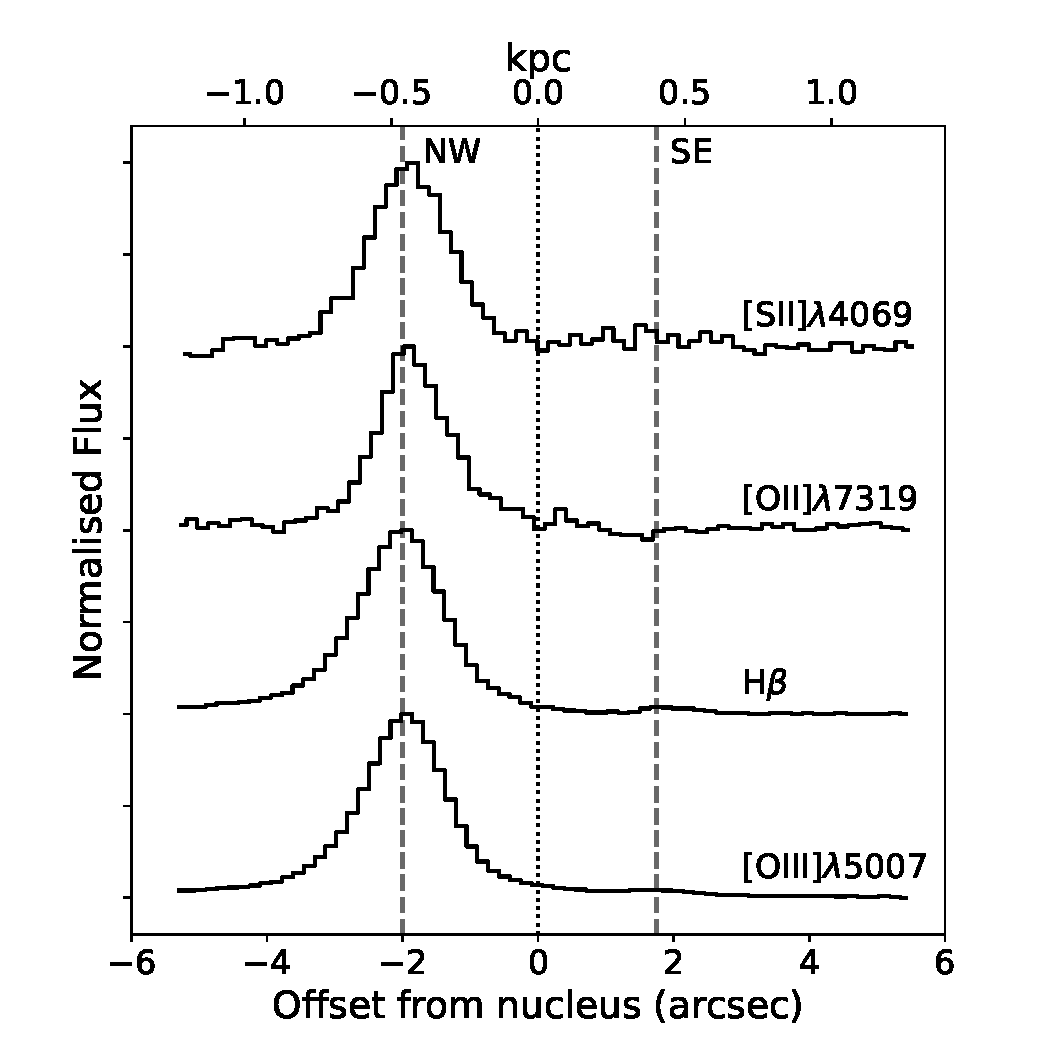
\includegraphics[width=0.7\linewidth]{figures/xshooter_ic5063/spatial_optical_labeled.pdf}
	\caption[Spatial distributions of the blue wings of the transauroral {[}OII{]} and {[}SII{]} lines, in addition to {[}OIII{]}$\lambda5007$ and H$\beta$ lines along the radio axis of IC\;5063.]{Spatial distributions of the blue wings (\mbox{$-$600\;\textless\;$v$\;\textless\;$-$400\;km\;s$^{-1}$}) of the transauroral [SII] and [OII] lines, H$\mathrm{\beta}$, and [OIII]$\lambda$5007 emission lines. The spatial flux distribution of the transauroral lines can be seen to closely follow those of [OIII] and H$\mathrm{\beta}$. The dotted line shows the position of the nucleus, and the dashed lines show the positions of the centroids of the NW and SE radio lobes, as measured from 24.8\;GHz imaging presented by \citet{Morganti2007}.}
	\label{fig: xshooter_ic5063: spatial_optical}
    \vspace*{1cm}
\end{figure}

Previous studies that make use of the transauroral lines to derive electron densities have been spatially unresolved (e.g. \citealt{Holt2011, Rose2018, Santoro2018, Spence2018, Santoro2020, Davies2020}), and it has not yet been verified that the transauroral lines are emitted by the same clouds as other key diagnostic lines such as [OIII]$\lambda$5007 and H$\mathrm{\beta}$ (see discussion in Section\;\ref{section: introduction: outflows: energetics: electron_densities}). However, from the Xshooter spectra presented here, it is found that the [OIII] models provide good fits to the lines used in this analysis, including the transauroral [SII] and [OII] doublets (Figure\;\ref{fig: xshooter_ic5063: o3_models_all_lines}). This demonstrates that these lines have similar profiles and thus similar kinematics, potentially indicating that they are emitted by the same cloud systems. To verify this, spatial slices of the blue wings of several key emission lines in the velocity range \mbox{$-$600\;\textless\;$v$ \;\textless\;$-$400\;km\;s$^{-1}$} were extracted from the two-dimensional spectra, avoiding any narrow components of the line profiles. Slices of continuum emission were also extracted, free from any emission lines, both blue-ward and red-ward of each emission line with slice widths of 20\;\AA. The two continuum slices were added and scaled to account for the different number of pixel columns extracted from the blue wing of each line --- the average continuum slice was then subtracted from the blue wing. The spatial position of the nucleus at the wavelength of each line was determined using Gaussian fits to the continuum spatial slices, and the peak positions of the extended emission line structures were then measured relative to this estimated nucleus position using Gaussian fits. Spatial flux distributions produced in this way are presented in Figure\;\ref{fig: xshooter_ic5063: spatial_optical}, and the peak centroid positions of the extended line emission from the Gaussian fits are given in Table\;\ref{tab: xshooter_ic5063: spatial_vis}.

From this analysis, it can be seen that the spatial flux profiles for the transauroral [OII] and [SII] lines are similar to those of the [OIII]$\lambda$5007 and H$\mathrm{\beta}$ lines. Furthermore, the values of the fitted Gaussian centroids for the peak of each line are consistent within 0.6\;pixels, a remarkable result given the known uncertainties from the Gaussian fitting process and the unknown systematic uncertainties from the continuum subtraction process, which will affect the lower-flux transauroral lines more than the brighter [OIII] and H$\mathrm{\beta}$ lines. In addition to the [OIII] models fitting the transauroral-line profiles well, this is taken as evidence that the transauroral lines are emitted in the same spatial locations as other key diagnostic lines. However, the possibility of the lines being emitted by different clouds within the same spatial apertures cannot be entirely ruled out.

\subsubsection{Transauroral-line diagnostics}
\label{section: xshooter_ic5063: properties_of_outflowing_gas: uvb_vis_analysis_and_results: transauroral_lines}

The high spectral resolution and wide wavelength coverage of the Xshooter observations allow the use of a technique first presented by \citet{Holt2011}, which employs the traditional and transauroral [OII] and [SII] lines to simultaneously derive values for electron density and reddening. This is done by comparing the following emission-line-flux ratios to those expected from photoionisation modelling:
\begin{align*}
TR([OII]) = F(3726 + 3729) / F(7319 + 7331), \\
TR([SII]) = F(4068 + 4076) / F(6717 + 6731).
\end{align*} 

A major advantage of this technique is that the \textit{total} line fluxes of the doublets are used for the ratios, instead of the flux ratios of lines \textit{within} the doublets (as is the case for traditional techniques of electron-density estimation) which are sensitive to blending effects at larger line widths. The [OIII] models were used as bases for the fits to the lines involved in the TR([OII]) and TR([SII]) ratios. In order to avoid additional issues due to degeneracy and blending owing to the complex kinematics, further constraints to the fits for a given kinematic component were applied in several ways. First, the widths of lines in a doublet were forced to be equal, and the wavelength separations between them were set to be those defined by atomic physics. Second, the intensity ratios of doublet lines were constrained in the following ways in order to ensure that the fits were not unphysical.
\begin{itemize}
	\item The ratios of the [OII]$\lambda\lambda$3726,3729, [SII]$\lambda\lambda$4049,4076, and [SII]$\lambda\lambda$6717,6731 doublets were forced to be within the range of their theoretical values \citep{Osterbrock2006, Rose2018}; if a measured intensity ratio was above or below this permitted range, it was forced to be the maximum or minimum allowed theoretical value, respectively.
	\item The intensity ratio of the [OII](7319/7330) ratio was set to be 1.24 because this ratio does not vary with density \citep{Rose2018}. Note that this doublet is actually two distinct doublets ([OII]$\lambda\lambda$7319,7320 and [OII]$\lambda\lambda$7330,7331); however, here they are modelled as single lines because their separation ($\sim$1\;{\AA}) is much lower than the widths of the narrowest kinematic components of the [OIII] models. Note that, while no broadening correction was made to account for the closely-spaced doublets, the [OIII] models still provided robust descriptions of the line profiles when considered as single lines (Figure \ref{fig: xshooter_ic5063: o3_models_all_lines}).
\end{itemize}

The \textsc{CLOUDY} photoionisation code (version C17.02: \citealt{Ferland2017}) was used to create single-slab, plane-parallel, radiation-bounded, and solar-composition models of photo-ionised gas with no dust depletion. The central photoionising continuum followed a power-law of shape $F_v \propto v^{-\alpha}$ between 10\;{\textmu}m and 50\;keV, with a spectral index of $\alpha=1.5$. This is close to the average optical-to-X-ray spectral index measured in radio-quiet AGN \citep{Zamorani1981, Miller2011}, and is consistent with photoionisation modelling of the emission-line ratios of the extended and nuclear NLRs in various samples of AGN (e.g. \citealt{Ferland1983}, \citealt{Robinson1987}). Ionisation parameters ($U$) were estimated for each aperture using estimated [OIII]/H$\mathrm{\beta}$ and [NII]/H$\mathrm{\alpha}$ line ratios with the relation presented by \citet{Baron2019b}: the resulting ionisation parameters were in the range \mbox{$-$2.90\;\textless\;log$U$\;\textless\;$-$2.45}. Therefore, log$U=-$2.75 was chosen for use in the \textsc{CLOUDY} models. The electron density of the modelled gas was varied by 0.1\;dex steps in the range \mbox{2.0\;\textless\;log$_{10}(n_\mathrm{e}$\;[cm$^{-3}$])\;\textless\;5.0}, and the CCM89 reddening law was used with $R_\mathrm{v}=3.1$ to redden these simulated TR ratios in order to create a grid with varying electron density and reddening. The resulting grid, along with the measured TR ratios in each aperture, is shown in Figure\;\ref{fig: xshooter_ic5063: tr_grid}, and the densities derived from this method are presented in Table\;\ref{tab: xshooter_ic5063: densities}. I note that these values were determined using a finer grid than is shown in Figure\;\ref{fig: xshooter_ic5063: tr_grid}.

\begin{figure}[!ht]
    \centering
	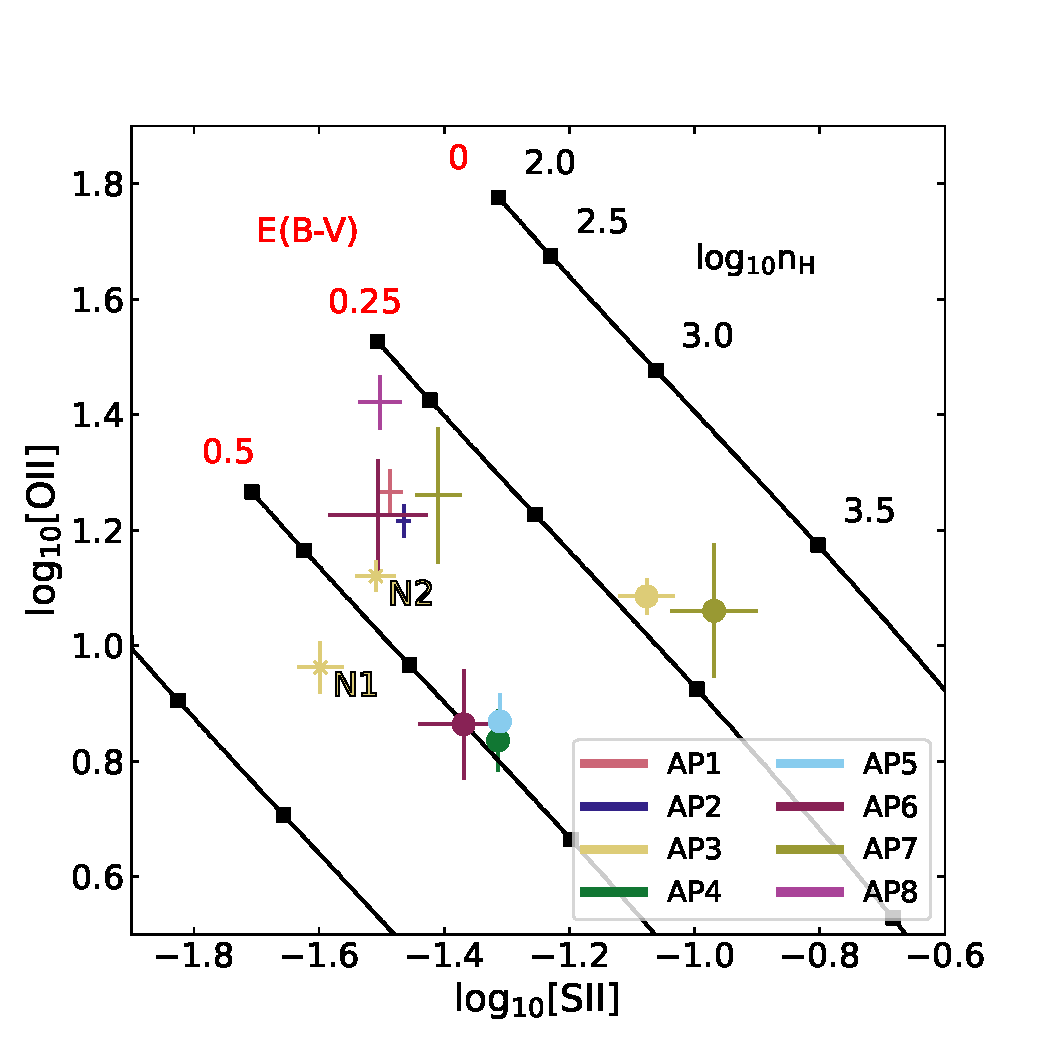
\includegraphics[width=0.75\linewidth]{figures/xshooter_ic5063/ddd_grid_zoomed.pdf}
	\caption[Transauroral {[}OII{]} and {[}SII{]} line ratio diagram for IC\;5063, showing both measured values and those predicted from photoionisation modelling.]{log$_{10}$ values of TR line ratios measured for the total narrow (crosses) and broad (circles) components in each aperture. Values for the total line profiles, as measured in apertures 4 and 5, are also shown as circles. The two narrow components in Aperture 3 are marked as `N1' and `N2'. Overlaid is a grid of simulated TR line ratios created using the \textsc{CLOUDY} photoionisation code (version C17.02, \citealt{Ferland2017}) for different values of electron density and reddened using the CCM89 reddening law, indicated by the joined series of black squares.}
	\label{fig: xshooter_ic5063: tr_grid}
\end{figure}

Using the transauroral line ratios, it is found that the broad components have significantly higher (\mbox{\textgreater\;3$\sigma$}) electron densities (\mbox{3.17\;\textless\;log$_{10}(n_\mathrm{e}$\;[cm$^{-3}$])\;\textless\;3.43}) than the narrow components (\mbox{2.12\;\textless\;log$_{10}(n_\mathrm{e}$\;[cm$^{-3}$])\;\textless\;2.59}) in all apertures where both are measured. In apertures 4 and 5 (where total line fluxes were used), the measured electron densities are consistent with those of the broad components in other apertures. Furthermore, in apertures where only a narrow component is measured (apertures 1, 2 and 8), densities similar to those of the narrow components in other apertures are found. The reddenings that are derived from the transauroral lines are moderately high (\mbox{0.17\;\textless\;E(B$-$V)$_{TR}$\;\textless\;0.51}), with no clear distinction between the values for narrow and broad components.

\begin{table*}
    \centering
	\def\arraystretch{1.5}
	\begin{tabular}{lcccc}
	\multirow{2}{*}{Component} & log$_{10}(n_\mathrm{e}$\;[cm$^{-3}$]) & log$_{10}(n_\mathrm{e}$\;[cm$^{-3}$]) & log$_{10}(n_\mathrm{e}$\;[cm$^{-3}$])  & log$_{10}(n_\mathrm{e}$\;[cm$^{-3}$])  \\ 
        & (TR) & ([OII]) & ([SII]) & ([ArIV]) \\
    \hline
	AP1 Narrow       & 2.53$^{+0.06}_{-0.07}$ & \textless\;2.13                                     & 1.97$^{+0.08}_{-0.10}$                    & 3.70$^{-0.27}_{+0.24}$      \\
		&	&	&	&	\\
	AP2 Narrow       & 2.65$^{+0.03}_{-0.04}$ & 2.02$^{+0.11}_{-0.14}$                    & \textless\;2.15                                     & \textless\;3.71                                        \\
	&	&	&	&	\\
	AP3 Narrow 1     & 2.59$^{+0.05}_{-0.05}$ & --- & --- & ---                   \\
	AP3 Narrow 2     & 2.55$^{+0.03}_{-0.03}$ & --- & --- & ---                  \\
	AP3 Broad        & 3.30$^{+0.05}_{-0.05}$ & --- & 2.84$^{+0.09}_{-0.09}$                    & ---    \\
	&	&	&	&	\\
	AP4 Total        & 3.25$^{+0.05}_{-0.05}$ & --- & ---  & 3.79$^{+0.18}_{-0.19}$   \\
&	&	&	&	\\
	AP5 Total        & 3.23$^{+0.04}_{-0.05}$ & --- & --- & \textless\;5.97 \\
&	&	&	&	\\
	AP6 Narrow       & 2.55$^{+0.16}_{-0.20}$ & --- & --- & ---   \\
	AP6 Broad        & 3.17$^{+0.09}_{-0.09}$ & --- & --- & ---    \\
&	&	&	&	\\
	AP7 Narrow       & 2.69$^{+0.15}_{-0.19}$ & --- & --- & ---    \\
	AP7 Broad        & 3.43$^{+0.09}_{-0.09}$ & --- & --- & ---    \\
&	&	&	&	\\
	AP8 Narrow       & 2.12$^{+0.14}_{-0.12}$ & 2.07$^{+0.11}_{-0.12}$  & 2.02$^{+0.14}_{-0.17}$ & \textless4.03  \\
	\end{tabular}
	\caption[Electron densities for the warm-ionised gas along the radio axis of IC\;5063, measured with the transauroral line technique, the traditional {[}SII{]} and {[}OII{]} line ratios, and the {[}ArIV{]}(4711/4740) ratio.]{Electron density values determined using the TR, traditional, and [ArIV] line ratios for the gas in IC\;5063. 3$\sigma$ upper limits are shown where the measured line ratio was not 3$\sigma$ from the lower or upper limit of the traditional line ratios. It was not possible to determine values for electron density using the traditional and [ArIV] line ratios in every aperture due to line blending and low signal relative to the continuum --- these cases are marked with a dash. Distances for each aperture are given in the same convention as Table\;\ref{tab: xshooter_ic5063: kinematics}.}
	\label{tab: xshooter_ic5063: densities}
\end{table*}

\begin{table*}[]
    \centering
	\def\arraystretch{1.5}
	\begin{tabular}{lcc}
	Component        &  E(B$-$V)$_\mathrm{TR}$      & E(B$-$V)$_{\mathrm{H\gamma}/\mathrm{H\beta}}$ \\ \hline
	AP1 Narrow       & 0.37$^{+0.02}_{-0.03}$ & 0.331$\pm$0.010   \\
	   &	&	\\
	AP2 Narrow       & 0.38$^{+0.02}_{-0.02}$ & 0.311$\pm$0.007   \\
	   &	&	\\
	AP3 Narrow 1     & --- & ---                   \\
	AP3 Narrow 2     & --- & ---                  \\
	AP3 Broad        & 0.22$^{+0.03}_{-0.03}$ & 0.215$\pm$0.017   \\
	   &	&	\\
	AP4 Total        & 0.48$^{+0.03}_{-0.03}$ & 0.507$\pm$0.026   \\
	   &	&	\\
	AP5 Total        & 0.46$^{+0.02}_{-0.02}$ & 0.342$\pm$0.019   \\
	   &	&	\\
	AP6 Narrow       & 0.40$^{+0.05}_{-0.05}$ & 0.172$\pm$0.029   \\
	AP6 Broad        & 0.50$^{+0.06}_{-0.05}$ & 0.399$\pm$0.062   \\
	   &	&	\\
	AP7 Narrow       & 0.33$^{+0.06}_{-0.07}$ & 0.265$\pm$0.016   \\
	AP7 Broad        & 0.17$^{+0.22}_{-0.07}$ & 0.270$\pm$0.037   \\ 
	   &	&	\\
	AP8 Narrow       & 0.30$^{+0.03}_{-0.03}$ & 0.270$\pm$0.029   \\
	\end{tabular}
    \caption[E(B$-$V) values for the warm-ionised gas along the radio axis of IC\;5063, measured with the transauroral line technique and the Balmer decrement method.]{Reddening values (E(B$-$V)) for the warm-ionised gas in each aperture, determined using both the transauroral-line-ratios (TR) and the H$\mathrm{\gamma}$/H$\mathrm{\beta}$ ratios with Case B recombination theory and the CCM89 reddening law.}
    \label{tab: xshooter_ic5063: reddenings}
\end{table*}

Note that the position of the TR line-ratio grid generated from photoionisation modelling potentially depends on the ionisation parameter, ionising continuum spectral index and metallicity used in the model. \citet{Santoro2020} show that varying the ionisation parameter in the range \mbox{$-$3.8\;\textless\;log$U$\;\textless\;$-$2} and gas metallicities in the range \mbox{0.5\;Z$_\odot$\;\textless\;$Z$\;\textless\;2\;$Z_\odot$} with different SED shapes can change the derived electron density values by 0.1--0.7\;dex and reddening values by 0.1--0.2 mag. However, for lower density clouds ($n_e$\;\mbox{\textless\;10$^4$\;cm$^{-3}$}) such as those measured here, the effect of varying these parameters on the electron density is reduced to 0.1--0.3\;dex. This corresponds to a maximum factor of two in derived electron density, which is much less than the potential order-of-magnitude inaccuracy incurred by using lower-critical-density diagnostics for higher-density clouds, as well as uncertainties associated with line blending within the traditional doublets.

\subsubsection{Traditional-line-ratio electron densities}
\label{section: xshooter_ic5063: properties_of_outflowing_gas: uvb_vis_analysis_and_results: trad_densities}

In addition to the electron densities determined using the transauroral technique, the traditional [OII](3726/3729) and [SII](6716/6731) emission line ratios and the higher-critical-density, higher-ionisation [ArIV](4711/4740) ratio were used to provide independent estimates of electron density, allowing the different techniques to be compared. The fluxes of the lines in each doublet were constrained using the [OIII] models, as shown in Figure\;\ref{fig: xshooter_ic5063: o3_models_all_lines}. It was not possible to fit certain doublets in some apertures due to line blending, and, in the case of the [ArIV] doublet, the low fluxes of the lines relative to the underlying stellar continua. Therefore, derived densities are not reported for these cases.

In order to ensure that the electron densities derived from the traditional ratios were accurate, it was required that the measured line ratios were 3$\sigma$ away from the theoretical lower and upper ratio limits (\citealt{Osterbrock2006}: \mbox{0.41\;\textless\;[OII]($3729/3726$)\;\textless\;1.50}, \mbox{0.30\;\textless\;[SII]($6717/6731$)\;\textless\;1.45}; \citealt{Wang2004}: \mbox{0.117\;\textless\;[ArIV]($4711/4740$)\textless\;1.50}). In several cases, the measured line ratios did not meet this criterion, as they were within $3\sigma$ of the ratio limit corresponding to low densities --- in this scenario, upper density limits were determined instead by using the value of the ratio that was $3\sigma$ away from the measured value.

Where it was possible to make robust measurements of these ratios, the \textsc{fivel} script \citep{Shaw1995} was used to calculate values for electron density. Doing so required an estimate of the electron temperature, which was determined for each component in each aperture using the [OIII](4959 + 5007)/4363 ratio (Section\;\ref{section: xshooter_ic5063: properties_of_outflowing_gas: uvb_vis_analysis_and_results: electron_temperatures}). The electron densities determined using all techniques discussed are shown in Table\;\ref{tab: xshooter_ic5063: densities}. 

Unfortunately, it was only possible to measure densities using all diagnostic methods for the narrow components in apertures 1, 2 and 8. In Aperture 8, all density estimates are consistent within the uncertainties, however, this is not the case for apertures 1 and 2, in which the TR ratios produce densities that are higher than those derived from the traditional [SII] and [OII] ratios, but lower than those from the [ArIV] ratio.

Considering the broad components, a traditional ratio ([SII]) can only be used to adequately measure an electron density in Aperture 3, where the value is significantly lower (\mbox{\textgreater\;3$\sigma$}) than the density found using the transauroral lines. The difference in the densities determined using the traditional ratio and the transauroral lines is approximately a factor of three in this case, and therefore Aperture 3 presents the best evidence for the TR lines producing higher densities than a traditional ratio for outflowing gas. In Aperture 4, the [ArIV] ratio gives a higher density than the TR lines, however, this difference is not significant to $3\sigma$; likewise, the [ArIV] density is higher than the value produced by the transauroral lines in Aperture 5, however, it should be noted that this is an upper limit.

\subsubsection{Recombination-line reddenings}
\label{section: xshooter_ic5063: properties_of_outflowing_gas: uvb_vis_analysis_and_results: balmer_decrement}

Determining precise values for reddening at different spatial positions is crucial for properly correcting the luminosities of emission lines which are used to determine outflow properties. In order to compare reddening values found using the transauroral-line technique to a more commonly used method, values for E(B$-$V) using the Balmer decrement were also determined. This was done by comparing the observed line flux ratio of the H$\mathrm{\gamma}$ and H$\mathrm{\beta}$ recombination lines to the intrinsic ratio expected from Case B recombination theory \citep{Osterbrock2006} and the CCM89 reddening law. The H$\mathrm{\alpha}$/H$\mathrm{\beta}$ ratios were not used to derive reddening values due to degeneracy issues related to blending between H$\mathrm{\alpha}$ and the [NII]$\lambda\lambda$6548,6583 doublet.

The results from the two methods of reddening estimation are shown in Table\;\ref{tab: xshooter_ic5063: reddenings}, and are shown plotted against each other in \mbox{Figure\;\ref{fig: xshooter_ic5063: tr_balmer_reddening}}. It is found that the transauroral-line method gives slightly higher values than using the H$\mathrm{\gamma}$/H$\mathrm{\beta}$ ratio, however, the two methods are consistent within 3$\sigma$ for all apertures except 2 and 5 (Table\;\ref{tab: xshooter_ic5063: reddenings}); both methods give a range of \mbox{0.17\;\textless\;E(B$-$V)\;\textless\;0.51}.

The H$\mathrm{\gamma}$/H$\mathrm{\beta}$ ratio can be sensitive to small errors in the subtraction of the underlying stellar continuum: \citet{Rose2018} show that a 10 per cent decrease in this ratio corresponds to a 60 per cent increase in the derived E(B$-$V) value. Therefore, while reddening values were derived using both the transauroral- and Balmer-line techniques for comparison, the values derived from the transauroral-line technique were used to de-redden the UVB+VIS spectra in all further analysis.

\begin{figure}[!t]
	\centering
	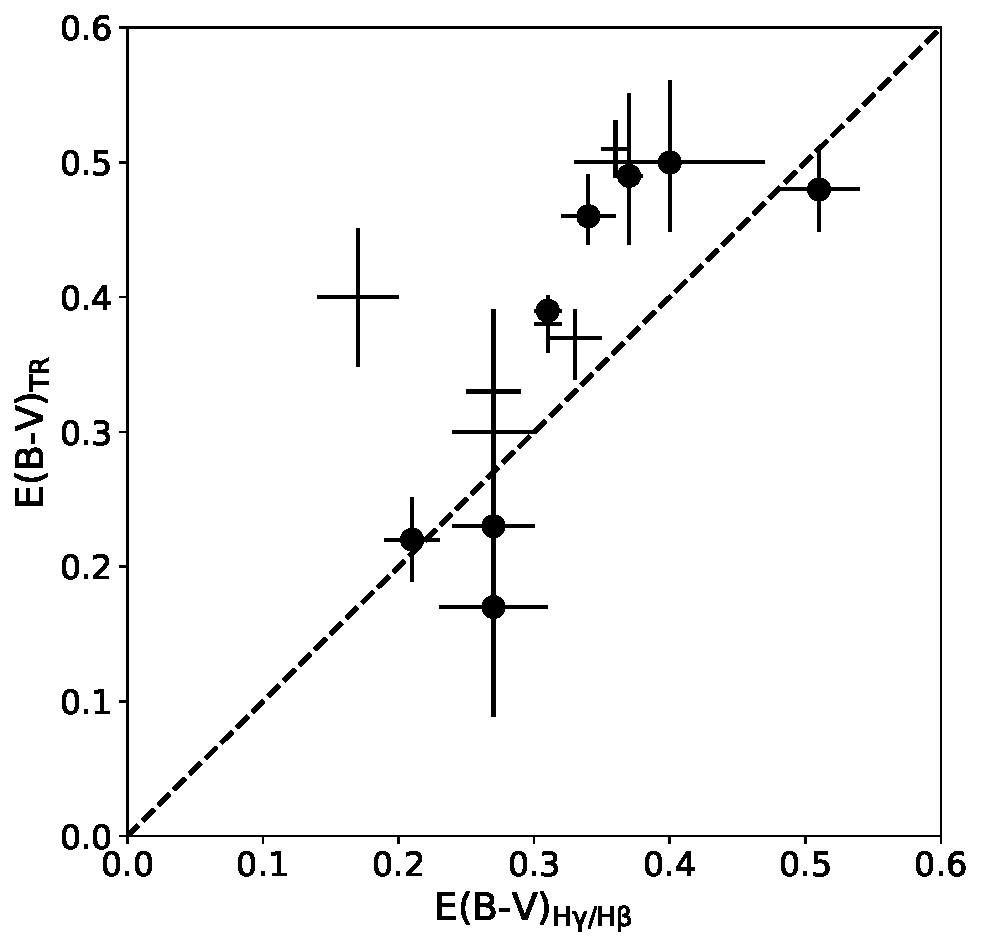
\includegraphics[width=0.75\linewidth]{figures/xshooter_ic5063/tr_balmer_reddening.pdf}
	\caption[Reddening values derived from the Balmer decrement plotted against values measured using the transauroral line technique.]{Reddening values derived from the Balmer decrement against values measured using the TR ratios. The black points represent the values measured in the various apertures and components, with broad components indicated by circles and narrow components by crosses, while the black dashed line shows the one-to-one relation. }
	\label{fig: xshooter_ic5063: tr_balmer_reddening}
\end{figure} 

\subsubsection{Electron temperatures and gas ionisation mechanisms}
\label{section: xshooter_ic5063: properties_of_outflowing_gas: uvb_vis_analysis_and_results: electron_temperatures}

Emission lines resulting from forbidden transitions of the O$^{+2}$ ion were used to determine electron temperatures --- this served as an initial probe of the ionisation mechanism of the outflowing and quiescent warm-ionised gas, since shock-ionised gas is expected to have a higher electron temperature than gas photoionised by AGN \citep{Fosbury1978, VillarMartin1999}. Note that the standard BPT diagrams were not used to investigate the ionisation mechanisms of the gas because the shock and photoionisation models overlap considerably in these diagrams (Section\;\ref{section: introduction: outflows: accleration_mechanisms: ionisation_and_excitation_mechanisms}, Figure\;\ref{fig: introduction: outflows: acceleration_mechanisms: bpt_diagram_photo_shock_ionisation}; \citealt{Zaurin2013}; \citealt{Santoro2018}), and the line profiles of H$\mathrm{\alpha}$ and the [NII]$\lambda\lambda$6548,6583 doublet are blended significantly in the apertures of interest. Electron temperatures were determined by using the extinction-corrected flux ratio [OIII](5007+4959)/4363 (using the [OIII] models to fit the lines) and transauroral-line-derived electron densities with the Lick Observatory \textsc{fivel} script. Values of electron temperature measured in this way for each kinematic component are presented in Table\;\ref{tab: xshooter_ic5063: temps}.

Using the [OIII](5007+4595)/4363 ratio, electron temperatures in the range \newline11500\;\textless\;$T_e$\;\textless\;14000\;K were found, with no clear distinction (\textgreater\;$3\sigma$) between broad and narrow components except in Aperture 3, in which the two narrow components present higher electron temperatures than the broad component.

	\begin{table}
	\def\arraystretch{1.5}
	\centering
	\begin{tabular}{cccc}
	Component & Distance (arcsec) & Distance (kpc) & Temperature (K) \\ \hline
	AP1 Narrow   & $-$4.72                                                       & $-$1.21                                                    & 11934$^{+169}_{-207}$                                     \\
		&	&	&	\\
	AP2 Narrow   & $-$3.44                                                       & $-$0.88                                                    & 13776$^{+145}_{-96}$                                      \\
	&	&	&	\\
	AP3 Narrow 1 & $-$1.84                                                       & $-$0.47                                                    & 14117$^{+350}_{-293}$                                     \\
	AP3 Narrow 2 & $-$1.84                                                       & $-$0.47                                                    & 13117$^{+185}_{-228}$                                     \\
	AP3 Broad    & $-$1.84                                                       & $-$0.47                                                    & 11564$^{+204}_{-160}$                                     \\
	&	&	&	\\
	AP4 Total    & 0                                                           & 0                                                        & 12578$^{+44}_{-44}$                                       \\
	&	&	&	\\
	AP5 Total    & 1.24                                                        & 0.32                                                     & 11810$^{+208}_{-164}$                                     \\
	&	&	&	\\
	AP6 Narrow   & 2.08                                                        & 0.53                                                     & 13921$^{+802}_{-666}$                                     \\
	AP6 Broad    & 2.08                                                        & 0.53                                                     & 12980$^{+941}_{-664}$                                     \\
	&	&	&	\\
	AP7 Narrow   & 3.04                                                        & 0.78                                                     & 11646$^{+457}_{-401}$                                     \\
	AP7 Broad    & 3.04                                                        & 0.78                                                     & 13680$^{+586}_{-517}$                                     \\
	&	&	&	\\
	AP8 Narrow   & 4.48                                                        & 1.15                                                     & 13537$^{+287}_{-282}$                                     \\ 
	\end{tabular}
	\caption[Electron temperatures for the warm ionised gas along the radio axis of IC\;5063, measured using the {[}OIII{]}(5007+4959)/4363 line ratio.]{Electron temperatures of the gas for each component in each aperture, derived using the [OIII](5007+4959)/4363 line ratio. The distances for each aperture are the same as given in Table\;\ref{tab: xshooter_ic5063: kinematics}.}
	\label{tab: xshooter_ic5063: temps}
\end{table}

To facilitate further comparisons with AGN photoionisation and shock models, the [OIII](5007/4363) against HeII$\lambda$4686/H$\mathrm{\beta}$ diagnostic diagram was produced (Figure\;\ref{fig: xshooter_ic5063: heii_hbeta}). The advantage of this diagram is that, not only are the shock and AGN-photoionisation models more clearly separated than in BPT diagrams, but it allows determinations of the extent to which the presence of matter-bounded clouds may play a role \citep{VillarMartin1999}. The AGN-photoionisation models were those generated by \textsc{Cloudy}, as described in Section\;\ref{section: xshooter_ic5063: properties_of_outflowing_gas: uvb_vis_analysis_and_results: transauroral_lines}, for a radiation-bounded, solar-composition (1\;Z$_\odot$), dust-free gas with an electron density of $n_\mathrm{e}=10^3$\;cm$^{-3}$ (based on the densities derived using the TR ratios) and a central ionising continuum that follows a power law of shape $F_\mathrm{v}$ $\propto$ $v^{-1.5}$. Note that the [OIII](5007/4363) and HeII4686/H$\mathrm{\beta}$ ratios depend on these parameters --- the effects of varying them are quantified and discussed in \mbox{Appendix \ref{appendix: heii_hb_oiii_photoionisation_modelling}}. The solar-composition shock models were taken from the library presented by \citet{Allen2008}, which was created using the \textsc{Mappings III} code. In \mbox{Figure\;\ref{fig: xshooter_ic5063: heii_hbeta}}, measured line ratios are plotted on this diagram for each aperture in which outflows are detected, along with the modelled \textsc{Cloudy} ratios for different ionisation parameters (in the range \mbox{$-$3.0\;\textless\;log$U$\;\textless\;$-$1.5}), and the pre-shock (precursor) and post-shock (pure-shock) models from \textsc{Mappings III} for a pre-shock gas density of 100\;cm$^{-3}$, magnetic fields of 1, 10 and 100\;$\mathrm{{\mu}G}$, and different shock velocities (ranging from 100--1000\;km\;s$^{-1}$).

By comparing the measured line ratios to those from the AGN-photoionisation and shock models, it can be seen that AGN photoionisation is dominant for both the outflowing and non-outflowing gas along the radio axis of IC\;5063. I highlight that, while pure AGN photoionisation requires a sub-solar metallicity ($\sim$0.5\;Z$_\odot$) and higher ionisation parameters than are measured here to explain some of the measured ratios, a different assumed spectral index would also help improve consistency with the AGN photoionisation models (see Appendix \ref{appendix: heii_hb_oiii_photoionisation_modelling}). Therefore, a plausible combination of these parameters exists that produces line ratios consistent with the measurements presented here. While some contribution from shocks cannot be ruled out, it should be noted that the [OIII](5007/4363) and HeII$\lambda$4686/H$\mathrm{\beta}$ ratios do not discriminate between broad and narrow components in this case (unlike the case presented by \citealt{VillarMartin1999}). Therefore, this is taken as evidence that both the quiescent and outflowing gas in the warm ionised phase are predominantly AGN-photoionised.

Moreover, moderate ($\sim0.10$--0.25) HeII$\lambda$4686/H$\mathrm{\beta}$ ratios and low-to-moderate [OIII] temperatures (\mbox{60\;\textless\;[OIII](5007/4363)\;\textless\;120}; 11500\;\textless\;$T$\;\textless\;14200\;K) are found for all components, both narrow and broad. These ratios rule out a major contribution from matter-bounded components \citep{Binette1996}.

\begin{figure}[!ht]
	\centering
	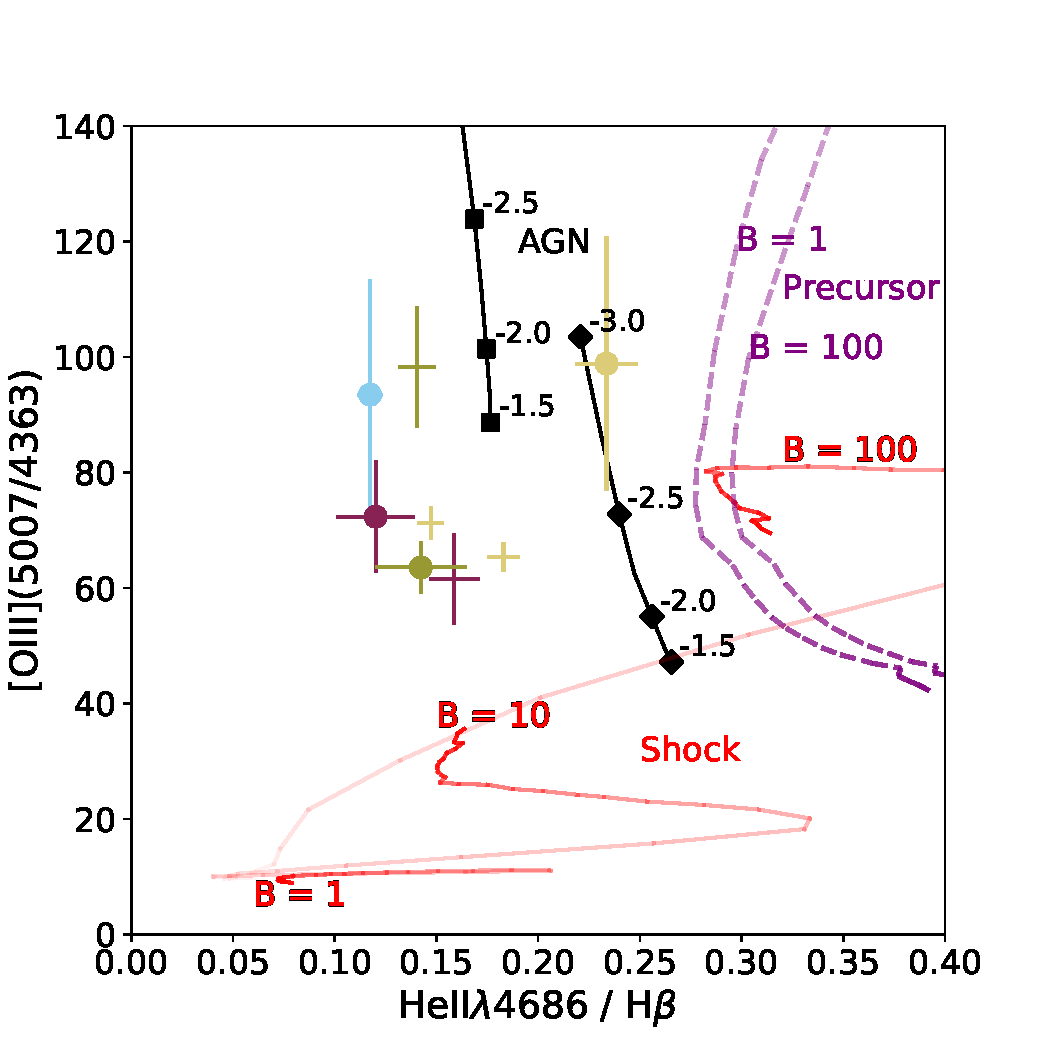
\includegraphics[width=0.7\linewidth]{figures/xshooter_ic5063/L_1Z.pdf}
	\caption[HeII$\lambda$4686/H$\mathrm{\beta}$ vs {[}OIII{]}(5007/4363) diagnostic diagram for the warm ionised gas in IC\;5063, including predicted values for photo- and shock-ionised gas.]{Measured HeII$\lambda$4686/H$\mathrm{\beta}$ and [OIII](5007/4363) line ratios for the outflowing gas in the Xshooter apertures --- the colour and marker scheme for each aperture is the same as in Figure\;\ref{fig: xshooter_ic5063: tr_grid}. Also plotted are AGN photoionisation models (black markers and lines) for different ionisation parameters (labelled) and spectral indices (squares: $\mathrm{\alpha}=1.5$; diamonds: $\mathrm{\alpha}=1.0$) of solar composition (1\;Z$_\odot$) gas of density $n_\mathrm{e}=10^3$\;cm$^{-3}$. Line ratios produced by shock-ionisation models taken from the \textsc{Mappings III} library presented by \citet{Allen2008} for gas with a pre-shock electron density of 100\;cm$^{-3}$, magnetic fields of 1, 10 and 100\;$\mu G$, and shock velocities ranging from 100--1000\;km\;s$^{-1}$ are shown as purple dashed lines (pre-shock/precursor gas) and red solid lines (post-shock gas). Lower shock velocities are shown with fainter lines, and higher shock velocities are shown with darker lines.}
	\label{fig: xshooter_ic5063: heii_hbeta}
\end{figure}

\subsubsection{Mass outflow rates and kinetic powers}
\label{section: xshooter_ic5063: properties_of_outflowing_gas: uvb_vis_analysis_and_results: energetics}

In order to facilitate comparisons between the results presented here, models of galaxy evolution, and previous observations of the different gas phases in IC\;5063, the derived properties of the outflows at different positions were used to derive mass outflow rates, kinetic powers, and coupling efficiencies for the warm-ionised outflows along the radio axis of IC\;5063.

The luminosities of the H$\mathrm{\beta}$ line for the broad component in each aperture were first calculated using
\begin{equation}
L(\mathrm{H\beta}) = F(\mathrm{H\beta})\times 4\pi D^2_L,
\end{equation}
where F(H$\mathrm{\beta}$) is the reddening-corrected flux of the H$\mathrm{\beta}$ line (measured from Gaussian fits using the [OIII] models), and $D_\mathrm{L}$ is the luminosity distance of IC\;5063. 

These luminosities were then used to determine the mass of an outflow in a given aperture using Equation \ref{eq: introduction: outflows: energetics: mout} with an assumed Case B recombination coefficient of $\alpha^\mathrm{eff}_\mathrm{H\beta}=3.03\times10^{-14}$\;cm$^{-3}$ (for $n_e=10^4$\;cm$^{-3}$ and $T_e=10^4$\;K) and electron densities derived from the TR ratios. Subsequently, the outflow masses derived in this way were used to produce mass outflow rate estimates for each aperture using Equation \ref{eq: introduction: outflows: energetics: mout_rate}, where $\Delta{R}$ was taken to be the width of a given aperture, and planar outflow geometry was assumed ($A=1$). As discussed in Section\;\ref{section: xshooter_ic5063: properties_of_outflowing_gas: uvb_vis_analysis_and_results: kinematics}, the outflow velocities ($v_\mathrm{out}$) were taken to be the difference between the percentile velocity ($v_\mathrm{p}$) of the broad component and the flux-weighted velocity ($v_\mathrm{w}$) of the narrow component in a given aperture (Table\;\ref{tab: xshooter_ic5063: kinematics}). 

Kinetic powers were estimated by using these mass outflow rates and kinematics with Equation\;\ref{eq: introduction: outflows: energetics: ekin}. I note that, since the outflow velocities were determined using percentile velocities (and it was assumed that the extremities of the emission-line wings represent the highest velocities along the LOS), the velocity width term of Equation\;\ref{eq: introduction: outflows: energetics: ekin} was not used (i.e. $\sigma$ was set to be zero). Finally, the resulting outflow kinetic powers were then compared to AGN bolometric luminosity to give coupling efficiencies ($\epsilon_\mathrm{f}$) using Equation\;\ref{eq: introduction: outflows: introduction: e_f}; the bolometric luminosity of IC\;5063 was taken to be 7.6$\times 10^{44}$\;erg\;s$^{-1}$ \citep{Nicastro2003, Morganti2007}. The resulting coupling efficiencies are presented in Figure\;\ref{fig: xshooter_ic5063: fkin} and Table\;\ref{tab: xshooter_ic5063: mout_fkin}. 

Low mass outflow rates (\mbox{\textless\;0.2\;M$_\odot$\;yr$^{-1}$}) and coupling efficiencies (\mbox{$\ll$\;0.5 per cent}) are found in all apertures --- much lower than those previously derived in some observational studies of samples of AGN (e.g. $\dot{M}_\mathrm{out}\sim10$--10,000\;M$_\odot$yr$^{-1}$: \citealt{Fiore2017}) and those required in galaxy-evolution models ($\epsilon_\mathrm{f}\sim0.5$--10\;per\;cent: e.g. \citealt{DiMatteo2005, Hopkins2010}). Furthermore, another set of coupling efficiencies was calculated (labelled $\epsilon_\mathrm{f}^{\prime}$) by determining the ratio of outflow kinetic power to the minimal jet power used in modelling of the jet-ISM interactions in IC\;5063 (P$_\mathrm{jet}$ = 10$^{44}$\;erg\;s$^{-1}$: \citealt{Mukherjee2018}). From this comparison, low values of $\epsilon_\mathrm{f}^{\prime}$ (\mbox{\textless\;0.001 per cent}) were produced, indicating that the kinetic power of the outflows accounts for an extremely small fraction of the total jet power and thus demonstrating the feasibility of jet-ISM interactions being the outflow acceleration mechanism.

\begin{figure}
	\centering
	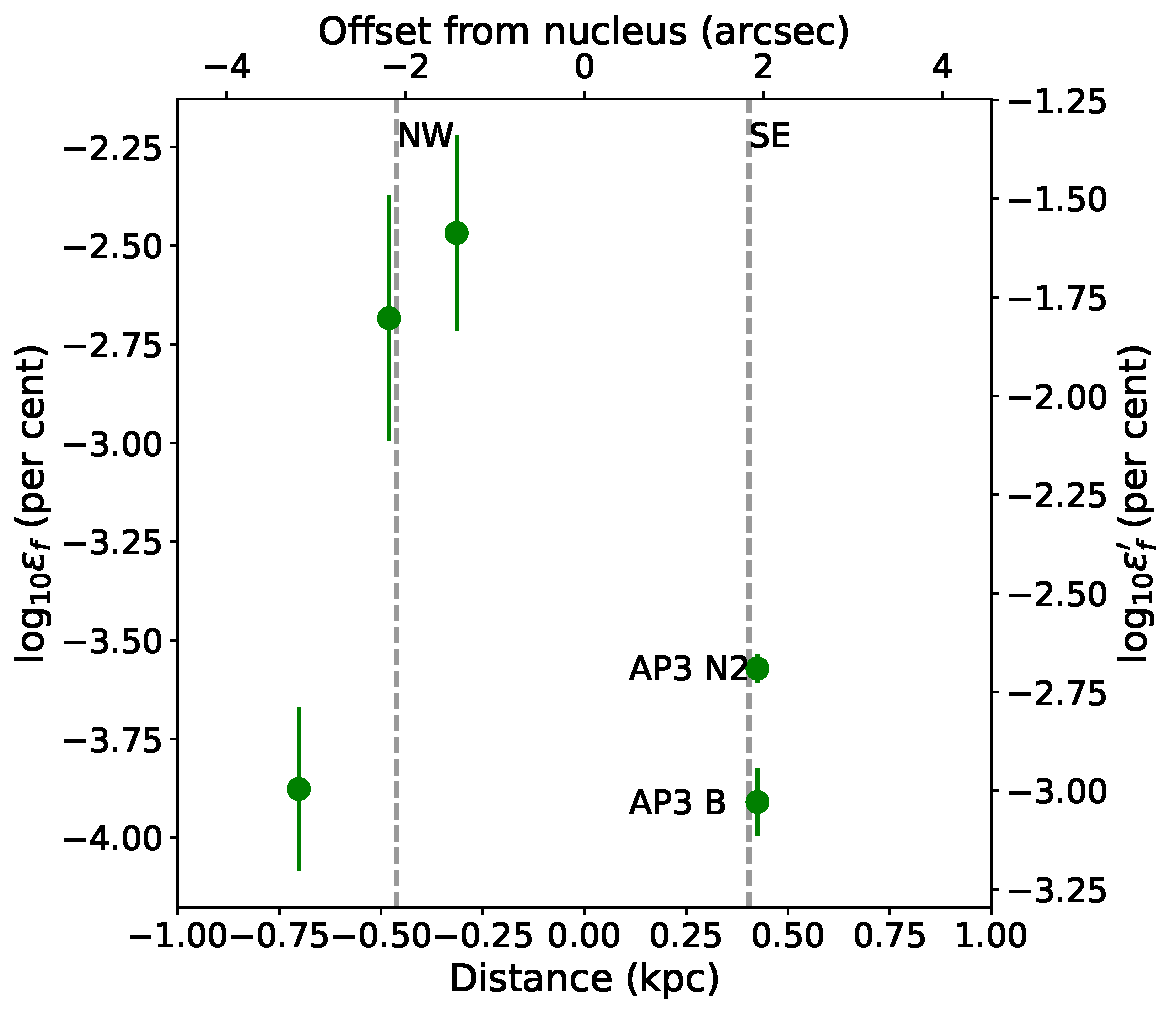
\includegraphics[width=0.8\linewidth]{figures/xshooter_ic5063/fkin.pdf}
	\caption[Outflow coupling efficiencies for the Xshooter apertures of IC\;5063, calculated for two cases: using the AGN bolometric luminosity, and for a jet of power $P_\mathrm{jet}=10^{44}$\;erg\;s$^{-1}$]{Percentage outflow coupling efficiencies in each aperture, calculated for two cases: using the nuclear bolometric luminosity of IC\;5063 given by \citet{Nicastro2003} and \citet{Morganti2007} ($\epsilon_\mathrm{f}=7.6\times 10^{44}$\;erg\;s$^{-1}$: left y-axis), and in the case that a jet of power P$_\mathrm{jet}=10^{44}$\;erg\;s$^{-1}$ \citep{Mukherjee2018} is the main driving mechanism ($\epsilon_\mathrm{f}^\prime$: right y-axis). The vertical dashed lines follow the same convention as Figure\;\ref{fig: xshooter_ic5063: velocities}, and the two kinematically-blueshifted components found in Aperture 3 (AP3 Broad and AP3 Narrow 2) are labelled.}
	\label{fig: xshooter_ic5063: fkin}
\end{figure}

\begin{table*}[!t]
	\renewcommand{\arraystretch}{1.5}
	\begin{tabular}{lcccc}
	Component    & $\dot{M}_\mathrm{out}$ (M$_\odot$yr$^{-1}$) & $\dot{E}_\mathrm{kin}$ (erg\;s$^{-1}$) & $\epsilon_\mathrm{f}$ (per cent) & $\epsilon_\mathrm{f}^\prime$ (per cent) \\ \hline
	AP3 Narrow 2 & 1.2$\pm$0.1 $\times 10^{-1}$              & 2.0$\pm$0.2 $\times10^{39}$  & 2.7$\pm$0.2 $\times 10^{-4}$   & 2.0$\pm$0.2 $\times 10^{-3}$          \\
	AP3 Broad    & 2.6$\pm$0.4 $\times10^{-2}$               & 9.4$\pm$1.8 $\times10^{38}$  & 1.2$\pm$0.2 $\times 10^{-4}$   & 9.4$\pm$1.8 $\times 10^{-4}$          \\ 
	AP5 Total    & 1.7$\pm$0.5 $\times 10^{-1}$               & 2.6$\pm$4.3 $\times10^{40}$  & 3.4$\pm$1.9 $\times 10^{-3}$   & 2.6$\pm$1.5 $\times 10^{-2}$          \\ 
	AP6 Broad    & 1.8$\pm$0.7 $\times 10^{-1}$              & 1.6$\pm$1.1 $\times10^{40}$  & 2.1$\pm$1.5 $\times 10^{-3}$   & 1.6$\pm$1.2 $\times 10^{-2}$          \\ 
	AP7 Broad    & 1.5$\pm$0.5 $\times 10^{-2}$              & 1.0$\pm$0.5 $\times10^{39}$  & 1.3$\pm$0.6 $\times 10^{-4}$   & 1.0$\pm$0.5 $\times 10^{-3}$          \\
	\end{tabular}
	\caption[Energetics for the warm ionised outflows in IC\;5063.]{Mass outflow rates, kinetic powers, and coupling efficiencies for the kinematic components associated with an outflow. The coupling efficiencies presented here are calculated using the nuclear bolometric luminosity of IC\;5063 given by \citet{Nicastro2003} ($\epsilon_\mathrm{f}=7.6\times 10^{44}$\;erg\;s$^{-1}$ ), and for a jet power of P$_\mathrm{jet} = 10^{44}$\;erg\;s$^{-1}$ ($\epsilon^\prime_\mathrm{f}$) as used in modelling by \citet{Mukherjee2018}.}
	\label{tab: xshooter_ic5063: mout_fkin}
\end{table*}


\newpage
\subsection{Analysis of the NIR apertures}
\label{section: xshooter_ic5063: properties_of_outflowing_gas: nir_analysis_and_results}

In order to obtain independent information about the gas ionisation/excitation and, potentially, acceleration mechanisms, the NIR spectra of the Xshooter observations of IC\;5063 were analysed separately.

First, it was found that the [OIII] models (Section\;\ref{section: xshooter_ic_5063: observations_and_data_reduction: emission_line_fitting}) did not describe the NIR emission-line profiles well: in many cases, the profiles were visibly different to those found in the UVB and VIS arms. Moreover, lines corresponding to different ionisation states (e.g. [FeII] and Pa$\mathrm{\beta}$) had differing line profiles within a given aperture. Therefore, unlike the UVB+VIS data, a line-profile model based on a single prominent emission line was not defined. Instead, each emission line was fit independently, and (as was done for the UVB+VIS spectra) Gaussian components were grouped into `broad' (\mbox{FWHM\;\textgreater\;500\;km\;s$^{-1}$}) or `narrow' (\mbox{FWHM\;\textless\;200\;km\;s$^{-1}$}) based on their line widths. Using the Gaussian fits produced in this way, the properties of several key, prominent emission lines in the NIR spectra were measured, namely [FeII]$\lambda$12570, [FeII]$\lambda$16400, Pa$\beta$, Br$\gamma$ and HeI$\lambda$10830 --- which trace the warm ionised phase --- and H$_2$1--0S(1)$\lambda$21218, which traces the warm molecular phase.

\subsubsection{The warm molecular gas phase}
\label{section: xshooter_ic5063: properties_of_outflowing_gas: nir_analysis_and_results: warm_molecular}

The H$_2 \lambda$21218 emission line can be used to probe the warm molecular gas phase, and comparing its line profile to those of forbidden and recombination lines allows for an investigation of the different outflow phases present in each aperture \citep{Tadhunter2014}. Broad ($\mathrm{FWHM}\sim500$\;km\;s$^{-1}$) components are seen in the H$_2 \lambda$21218 profiles in all apertures where outflowing gas is detected in [OIII] emission (consistent with the NIR observations of \citealt{Tadhunter2014}). Interestingly, the blueshifted narrow component in Aperture 3 seen in the optical line profiles (`AP3 Narrow 2') is absent in the H$_2 \lambda$21218 line profile (Figure\;\ref{fig: xshooter_ic5063: ap3_oiii_h2}), although it is present in the [FeII] and NIR recombination line profiles. This indicates that excited warm-molecular gas is not kinematically associated with the blueshifted component in Aperture 3.

\begin{figure}[!ht]
	\centering
	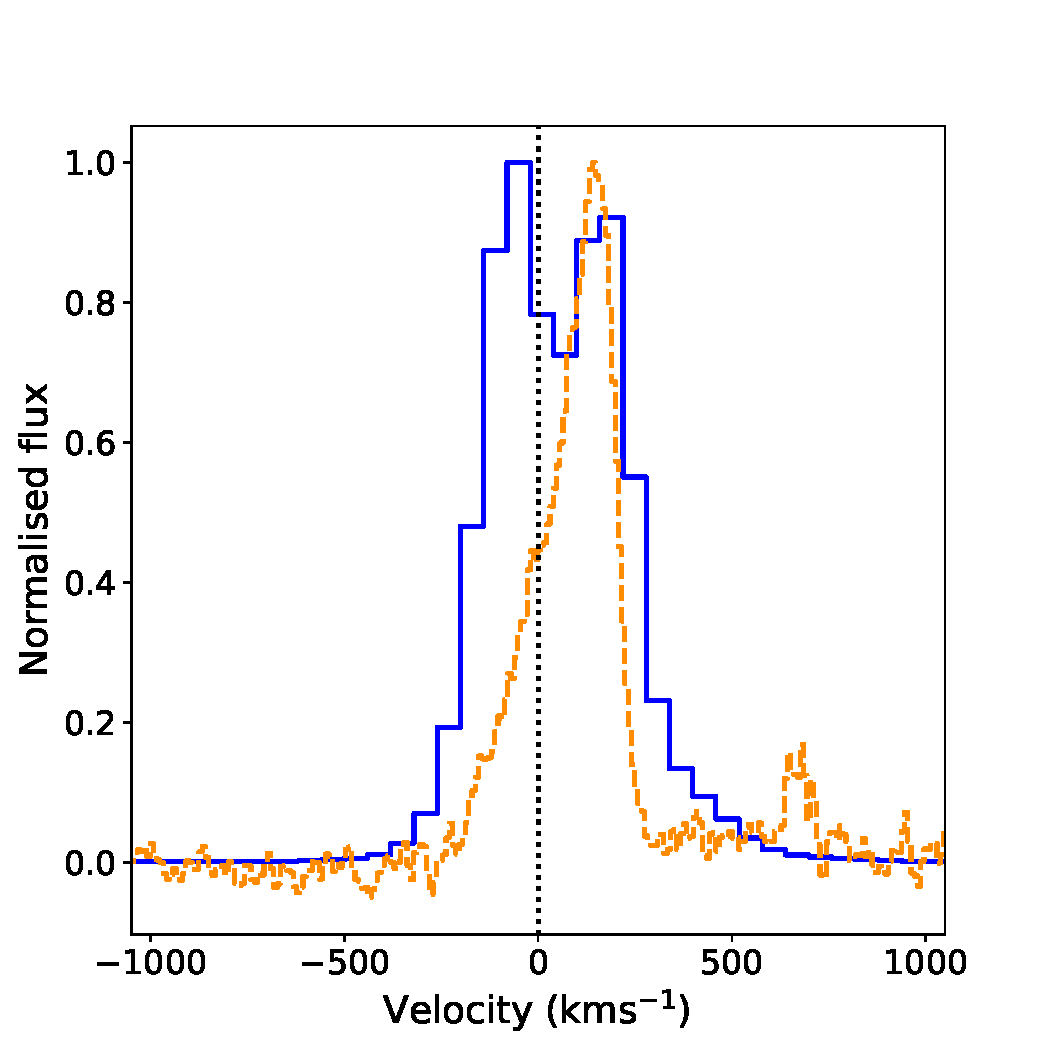
\includegraphics[width=0.7\linewidth]{figures/xshooter_ic5063/ap3_oiii_h2.pdf}
	\caption[Velocity profiles of for the {[}OIII{]}$\lambda$5007 and H$_2$1--0S(1)$\mathrm{\lambda}$21218 lines at the position of the SE radio lobe of IC\;5063.]{Velocity profiles for the [OIII]$\lambda$5007 (blue solid line) and \mbox{H$_2$1--0S(1)$\mathrm{\lambda}$21218} (orange dashed line) lines in Aperture 3. While a broad component --- representing outflowing gas --- is seen in both lines, the blueshifted narrow component seen in the [OIII] line profile (`AP3 Narrow 2'), emitted by the warm-ionised gas, is not present in the warm-molecular H$_2$ emission. Note that the [OIII]$\lambda$5007 line lies within the VIS Xshooter arm, and has been resampled to a wavelength step of 1\AA/pixel.}
	\label{fig: xshooter_ic5063: ap3_oiii_h2}
\end{figure}

\subsubsection{Ionisation and excitation of the near-infrared [FeII], Pa$\mathrm{\beta}$ and H$_2$ lines}
\label{section: xshooter_ic5063: properties_of_outflowing_gas: nir_analysis_and_results: excitation}

In order to supplement the investigation of the dominant outflow ionisation mechanism presented in Section\;\ref{section: xshooter_ic5063: properties_of_outflowing_gas: uvb_vis_analysis_and_results: electron_temperatures}, flux ratios of the [FeII]$\lambda$12570, [FeII]$\lambda$16400, and H$_2 \lambda$21218 emission lines and NIR recombination lines \citep{Rodriguez-Ardila2005, Riffel2013a, Colina2015, Riffel2021} were measured. In particular, I made use of the [FeII]$\lambda$12570/Pa$\mathrm{\beta}$ vs H$_2\lambda$21218/Br$\mathrm{\gamma}$ diagnostic diagram (see discussion in Section\;\ref{section: introduction: outflows: accleration_mechanisms: ionisation_and_excitation_mechanisms}) with the limits presented by \citet{Riffel2013a} and \citet{Riffel2021} that separate star-forming galaxies (SF), AGN and high line ratio (HLR) objects. The HLR region of the [FeII]$\lambda$12570/Pa$\mathrm{\beta}$ vs H$_2\lambda$21218/Br$\mathrm{\gamma}$ diagram contains objects such as Supernova Remnants (SNRs) and Low Ionisation Nuclear-Emission line Regions (LINERs; \citealt{Heckman1980}); objects for which photoionisation alone cannot explain the measured line ratios.

The line ratios of the different kinematic components in each aperture are shown plotted on this diagnostic diagram in Figure\;\ref{fig: xshooter_ic5063: feii_pab}, and are listed in Table\;\ref{tab: xshooter_ic5063: nir_ratios}. It is striking that the broad components of the NIR emission line profiles have higher H$_2\lambda$21218/Br$\mathrm{\gamma}$ ratios relative to the narrow components, with the broad components falling in the HLR region and the narrow components falling within the AGN region. Considering that the H$_2\lambda$21218/Br$\mathrm{\gamma}$ ratio probes the excitation of the warm-molecular gas, this indicates that the narrow components of this phase are predominately AGN-excited, while the broad components have composite shock-AGN excitation. In contrast, there is no clear difference in the [FeII]$\lambda$12570/Pa$\mathrm{\beta}$ ratios of the broad and narrow components, indicating that the quiescent and outflowing warm-ionised gas is predominantly AGN-photoionised (consistent with the results of Section\;\ref{section: xshooter_ic5063: properties_of_outflowing_gas: uvb_vis_analysis_and_results: electron_temperatures}).

\begin{figure}[!ht]
	\centering
	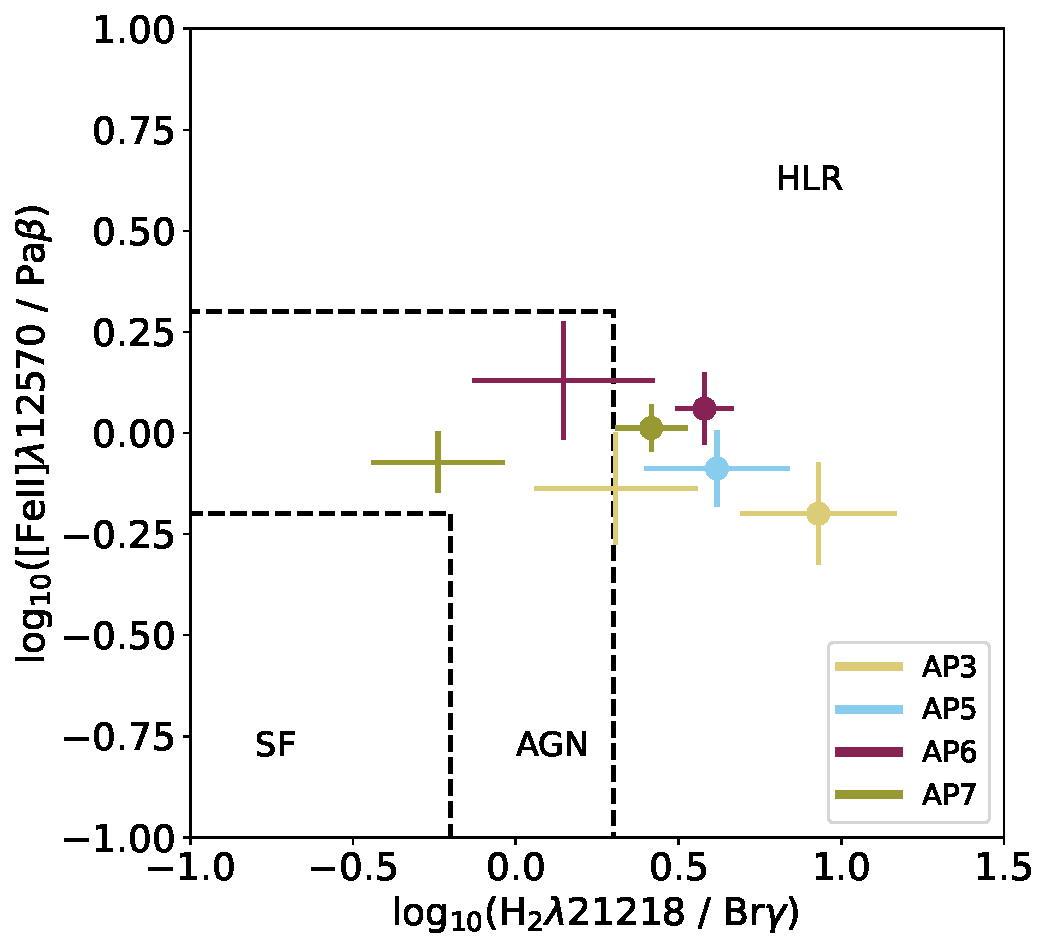
\includegraphics[width=0.75\linewidth]{figures/xshooter_ic5063/feii_pab.pdf}
	\caption[{[}FeII{]}$\lambda$12570/Pa$\mathrm{\beta}$ vs H$_2 \lambda$21218/Br$\mathrm{\gamma}$ NIR diagnostic diagram for the warm-ionised and warm-molecular NLR gas in IC\;5063.]{{[}FeII{]}$\lambda$12570/Pa$\mathrm{\beta}$ vs H$_2 \lambda$21218/Br$\mathrm{\gamma}$ NIR diagnostic diagram for the warm-ionised and warm-molecular NLR gas in IC\;5063 \mbox{(crosses: narrow components; circles: broad components)}, with regions defined by \citet{Riffel2021}: `SF' denotes observed line ratios which are associated with ionisation/excitation from star formation; `AGN' denotes line ratios which are associated with the central regions of AGN, and `HLR' denotes values higher than those observed from AGN-photoionisation/excitation alone. It has been proposed that line ratios in the HLR region indicate a contribution from shock-excitation, either from supernovae (SNe) or jet-ISM interactions. For IC\;5063, kinematic components associated with outflows fall within the HLR, with the quiescent components falling within the AGN region. The colour and marker scheme is the same as in Figure\;\ref{fig: xshooter_ic5063: tr_grid}.}
	\label{fig: xshooter_ic5063: feii_pab}
\end{figure}

\begin{table*}
	\centering
	\renewcommand{\arraystretch}{1.5}
	\begin{tabular}{lccc}
	Component    & H$_2\lambda$21218/Br$\mathrm{\gamma}$ & [FeII]$\lambda$12570/Pa$\mathrm{\beta}$ & [FeII]$\lambda$16400/Br$\mathrm{\gamma}$ \\ \hline
	AP3 Narrow 1 & 2.0$\pm$1.2    & 0.7$\pm$0.2                   & 4.5$\pm$2.5                  \\
	AP3 Broad    & 8.5$\pm$4.7    & 0.6$\pm$0.2                   & 3.1$\pm$1.8                  \\
		&	&	&	\\
	AP5 Total    & 4.2$\pm$2.1    & 0.8$\pm$0.2                   & 5.8$\pm$3.2                  \\
	&	&	&	\\
	AP6 Narrow   & 1.4$\pm$0.9    & 1.4$\pm$0.5                   & 3.6$\pm$2.2                  \\
	AP6 Broad    & 3.8$\pm$0.8    & 1.2$\pm$0.2                   & 6.5$\pm$1.6                  \\
	&	&	&	\\
	AP7 Narrow   & 0.6$\pm$0.3    & 0.9$\pm$0.2                   & 5.3$\pm$1.3                  \\ 
	AP7 Broad    & 2.6$\pm$0.7    & 1.0$\pm$0.1                   & 4.1$\pm$1.2                  \\
	\end{tabular}
	\caption[Ratios of NIR H$_2$ and {[}FeII{]} emission lines to recombination lines for the outflows in IC\;5063.]{Ratios of NIR H$_2$ and [FeII] emission lines to recombination lines for the components that are taken to represent outflowing gas. These values are shown on the [FeII]$\lambda$12570/Pa$\mathrm{\beta}$ vs H$_2\lambda$21218/Br$\mathrm{\gamma}$  diagnostic plot in Figure\;\ref{fig: xshooter_ic5063: feii_pab}, which is used to investigate the excitation mechanisms of the outflowing gas.}
	\label{tab: xshooter_ic5063: nir_ratios}
\end{table*}


\clearpage
\section{Discussion}
\label{section: xshooter_ic5063: discussion}

The results presented in Section\;\ref{section: xshooter_ic5063: properties_of_outflowing_gas} provide evidence for outflowing gas at the NW and SE radio lobes of IC\;5063 --- driven by jet-ISM interactions --- in agreement with the findings of previous studies (e.g. \citealt{Morganti2007, Tadhunter2014, Morganti2015}). This section discusses the relationship between the different gas phases at the NW lobe in detail, investigates which outflow phase is dominant in terms of mass and kinetic power through comparison to previous observations, and proposes a physical relation between the different gas phases and components along the radio axis. Finally, the implications of these findings for the transauroral-line technique of deriving electron densities are discussed.

\subsection{Placing the warm-ionised outflows at the NW lobe in a multi-phase context}
\label{section: xshooter_ic5063: discussion: multiphase}

\subsubsection{Kinematics of the different gas phases}
\label{section: xshooter_ic5063: discussion: multiphase: kinematics}

The [OIII] kinematics observed along the radio axis in IC\;5063 are consistent with a combination of regular gravitational disk rotation (traced by the narrow components, with the exception of the `Narrow 2' component in Aperture 3) and outflows of velocity 300\;\textless\;$v_\mathrm{out}$\;\textless\;700\;km\;s$^{-1}$ (traced by the broad components). As noted in previous work, the close association between highly-disturbed emission-line kinematics and the radio structure provides strong evidence that the warm-gas outflows are driven by the radio jet (e.g. \citealt{Morganti2007}, \citealt{Tadhunter2014}).

Kinematically, the results reported here for the warm ionised phase differ from what has previously been found for the cold-molecular gas. Here, extreme warm-ionised outflow kinematics are found at several positions along the radio axis, including the regions between the nucleus and the centroids of the radio lobes, whereas previous observations for the cold molecular phase --- as traced by CO emission lines --- find more extreme kinematics at the outer limit of NW lobe than elsewhere \citep{Morganti2015, Oosterloo2017}. In the two-dimensional Xshooter spectra for the warm-ionised gas (Figure\;\ref{fig: xshooter_ic5063: o2_pv_diagram}), there are indeed high-velocity blue wings extending to $v\sim1000$\;km\;s$^{-1}$ at the NW lobe, consistent with what is seen for the cold molecular phase. However, unlike the cold molecular phase, the warm-ionised gas profiles also have red wings extending to $v\sim800$\;km\;s$^{-1}$ at the position of the SE lobe. Most strikingly, the most extended velocity wings of the warm ionised phase, redshifted up to a maximum velocity of $\sim$1500\;km\;s$^{-1}$ at zero intensity, are found at a location \textit{between} the nucleus and the centroid of the NW lobe. The spatial centroid of this wing between \mbox{1000\;\textless\;$v$\;\textless\;1500\;km\;s$^{-1}$}, as measured by Gaussian fits to the continuum-subtracted spatial flux profile (as in Section\;\ref{section: xshooter_ic5063: properties_of_outflowing_gas: uvb_vis_analysis_and_results: spatial_distributions}) of the [NII]$\lambda$6583 line, lies 1.41\;arcsec north-west of the continuum centroid, or $\sim$0.6\;arcseconds (0.14\;kpc) closer to the nucleus than the centroid of the NW lobe.

The kinematics of the warm molecular phase, as traced with the H$_2\lambda$21218 emission, follow the warm-ionised kinematics. A blue velocity wing is seen to extend to $v\sim1000$\;km\;s$^{-1}$ at the centroid of the NW lobe, and a red wing extends to $v$\;\textgreater\;1000\;km\;s$^{-1}$ between this position and the nucleus (Figure\;\ref{fig: xshooter_ic5063: ap56_h2_velocity_profile}). This feature may extend to higher velocities, potentially up to $v\sim1500$\;km\;s$^{-1}$ (as seen in the warm-ionised gas), but blending with the continuum makes it difficult to determine the true velocity extent. These observed H$_2\lambda$21218 kinematics are also consistent with previous observations of the warm molecular phase by \citet{Tadhunter2014}.

The kinematics observed in the warm ionised and molecular phases can be explained by an expanding hemispherical bow shock or bubble, the tip of which coincides with --- or extends slightly beyond --- the centroid of the NW lobe. Considering that this structure would be seen side-on, the highest velocity widths are expected closer to the nucleus than the centroid of the lobe due to projection effects (i.e. the gas moving along the observer's line of sight). This is consistent with the highest observed velocities being between the nucleus and the outer limit of the NW lobe. Likewise, lower projected velocities would be found at the centroid of the lobe (closer to the tip of the bow shock), as the outflowing gas there would be moving in a direction that is close to the plane of the sky. The Xshooter observations are also consistent with the kinematics seen in hydrodynamic modelling of IC\;5063 for a jet of power P$_\mathrm{jet}=10^{44-45}$\;erg\;s$^{-1}$ propagating through the disk, as presented by \citet{Mukherjee2018}, where red- and blue-shifted line wings are seen at all locations where the radio source is interacting with the ISM in the galaxy's disk.

\begin{figure*}[!p]
	\centering
	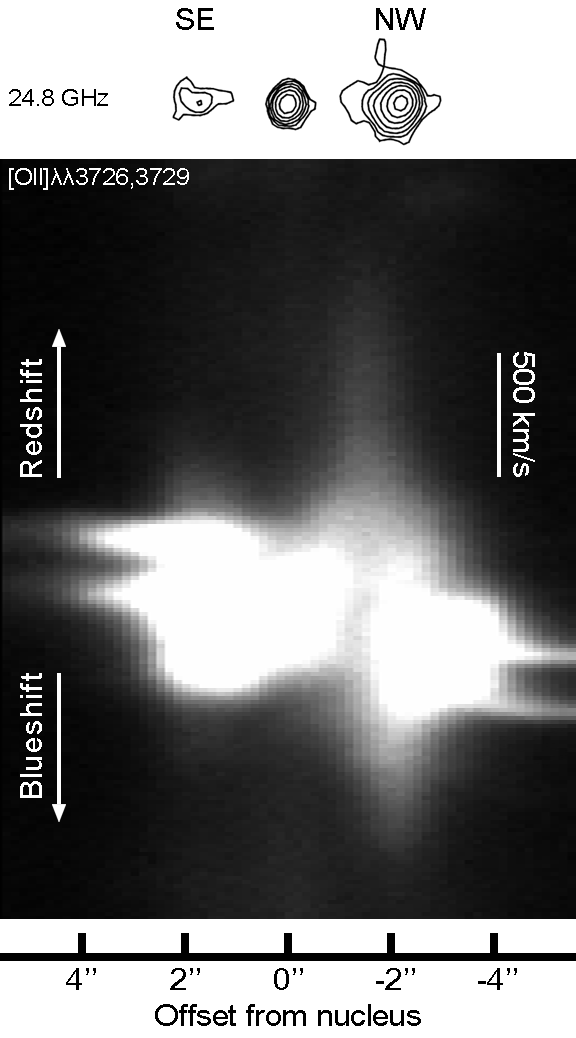
\includegraphics[width=0.7\linewidth]{figures/xshooter_ic5063/oii_h2_pv_diagram_3.png}
	\caption[Two-dimensional position-velocity profile of the {[}OII{]}$\lambda\lambda$3726,3729 doublet along the radio axis of IC\;5063, and corresponding 24.8\;GHz continuum contours.]{Two-dimensional position-velocity profile of the [OII]$\lambda\lambda$3726,3729 doublet. Here, the spatial direction is horizontal and the velocity (spectral) direction is vertical. Corresponding 24.8\;GHz continuum imaging by \citet{Morganti2007} is shown above the profile, indicating the shape and extent of the radio structure. The velocity scale bar represents a shift of $v=500$\;km\;s$^{-1}$. Very broad velocity wings can be seen at several locations, including at the centroids of the SE and NW lobes, with the most extended being a $v\sim1500$\;km\;s$^{-1}$ red wing between the nucleus and the centroid of the NW lobe.}
	\label{fig: xshooter_ic5063: o2_pv_diagram}
\end{figure*}

The difference in observed kinematics between the warm- and cold-molecular gas may be explained if the different molecular phases constitute a post-shock cooling sequence, as has been previously proposed to explain multi-phase outflow kinematics (see Section\;\ref{section: introduction: outflows: energetics: multi-phase}; \citealt{VillarMartin1999, Zubovas2014, Tadhunter2014}). In this scenario, the warm H$_2$ emission represents a transition phase, emitted as gas cools behind the shock through $T\sim2000$\;K, and has a constant mass and luminosity, assuming material passes through the shock at a constant rate. As the gas cools further, it enters the cold molecular phase, which emits the CO emission lines --- this represents the end-state of the cooling sequence. Assuming that the conditions for cold-molecular gas formation are met, and the molecular gas is not destroyed by AGN radiation, the ratio of cold-molecular gas (traced by CO emission) to warm-molecular gas (traced by H$_2$ emission) will thus increase as a function of time. In this scenario, if the gas seen in projection in-between the nucleus and the maximum extent of the NW radio lobe has only just started to enter the shock, it is plausible that not enough gas has yet accumulated in the cold molecular phase to be detectable via its CO emission. In contrast, gas may have been entering the shock at the tip of the hemispherical bow shock (the maximum extent of the NW lobe) for longer, allowing more time for CO-emitting cold-molecular gas to accumulate. This would explain why disturbed kinematics are seen at the centroid of the NW radio lobe for all phases, but only the warmer phases show more extreme kinematics in between this location and the nucleus.



\begin{figure}[!t]
	\centering
	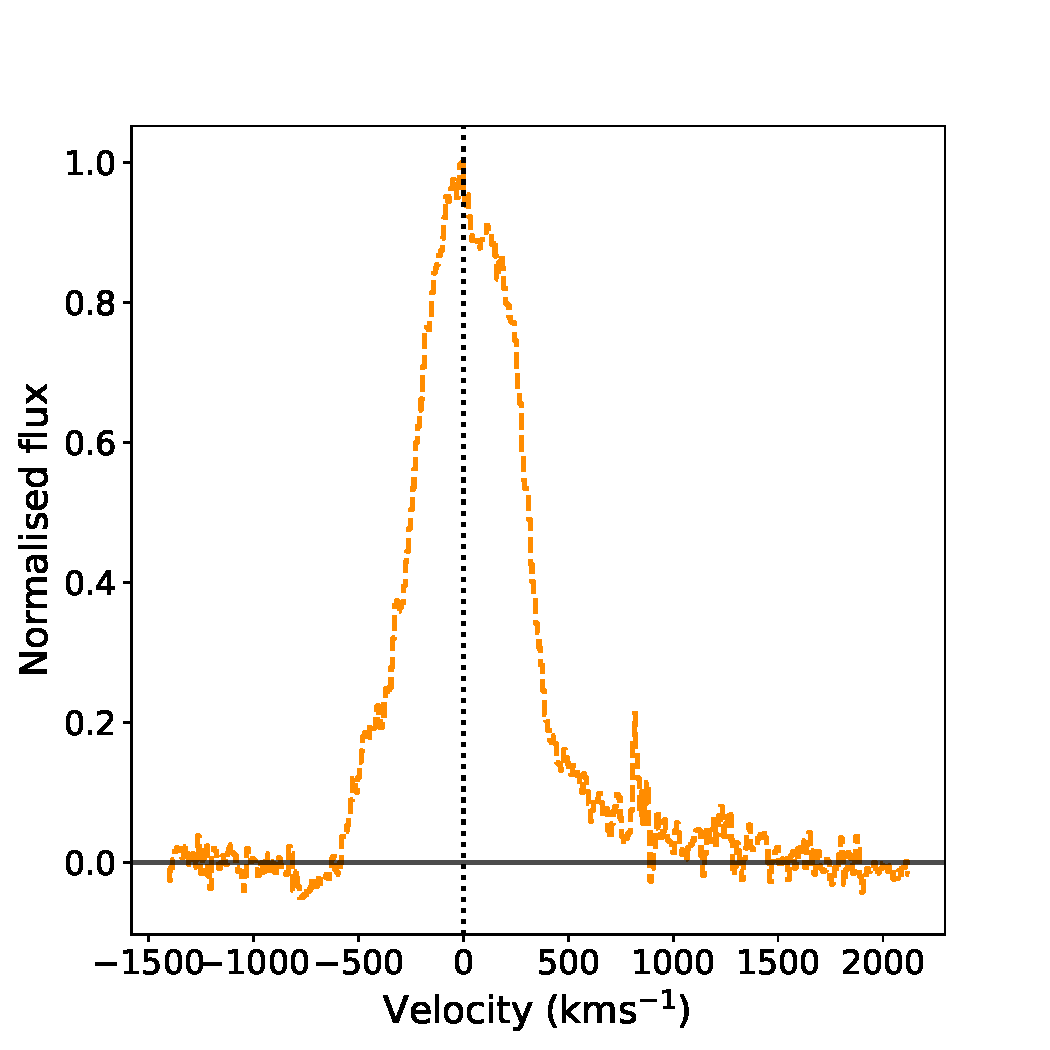
\includegraphics[width=0.7\linewidth]{figures/xshooter_ic5063/ap56_h2_velocity_profile.pdf}
	\caption[Velocity profile of the H$_2\lambda$21218 emission line at the location between the nucleus and outer extent of the NW radio lobe in IC\;5063.]{The velocity profile of the H$_2\lambda$21218 (dashed orange) line in the combined apertures 5 and 6, corresponding to the location between the nucleus and the outer extent of the NW radio lobe (Figure\;\ref{fig: xshooter_ic5063: apertures}). The dotted black vertical line represents a velocity of 0\;km\;s$^{-1}$, while the solid black horizontal line shows the continuum level. A red velocity wing extending to $v$\;\textgreater\;1000\;km\;s$^{-1}$ can be seen, consistent with the kinematics of the warm ionised phase (Figure\;\ref{fig: xshooter_ic5063: o2_pv_diagram}).}
	\label{fig: xshooter_ic5063: ap56_h2_velocity_profile}
\end{figure}

\subsubsection{Energetics of the multi-phase outflows}
\label{section: xshooter_ic5063: discussion: multiphase: energetics}

In order to ensure that the mass outflow rates and kinetic powers of the previously-observed neutral atomic and cold molecular phases are consistent with the results presented here for the warm ionised phase --- and to properly take into account results of the cold-molecular gas kinematics \citep{Morganti2015, Oosterloo2017} --- here, I recalculate values from past studies of IC\;5063 with a consistent methodology.

First, the mass outflow rate of the neutral-atomic (HI) outflow at IC\;5063's NW lobe was calculated using
\begin{equation}
    \dot{M}_\mathrm{out} = 30\cdot\frac{\Omega}{4\pi}\cdot\frac{r_\ast}{1\;\mathrm{kpc}}\cdot\frac{N_\mathrm{H}}{10^{21}\;\mathrm{cm}^{-2}}\cdot\frac{v_\mathrm{out}}{300}
\label{eq: xshooter_ic5063: appendix_hi_mout}
\end{equation}
from \citet{Morganti2005} (following the methodology given in \citealt{Heckman2002} and \citealt{Rupke2002}), where $N_\mathrm{H}$ is the column density of the gas and $\Omega$ is the solid angle through which the gas is flowing at a radius $r_\ast$ with a velocity of $v_\mathrm{out}$. Using the values and assumptions given in \citet{Morganti2005} --- namely that \mbox{$\Omega=\pi$}, \mbox{$r_\ast=0.4$\;kpc}, $N_\mathrm{H}=10\times10^{21}$\;cm$^{-2}$, and $v_\mathrm{out}=$ full width at zero intensity $\mathrm{(FWZI)}/2=350$\;km\;s$^{-1}$ --- a mass outflow rate of 35\;M$_\odot$\;yr$^{-1}$ was determined.

An important assumption made here is that the gas is outflowing through a solid angle of $\pi$, which is highly uncertain. Moreover, taking $v_\mathrm{out}$ = $\mathrm{FWZI}/2$ may underestimate the true outflow velocity in this case, since much of the blueshifted absorption in the HI 21\;cm profile of the NW lobe in IC\;5063 is concentrated close to the maximum blueshifted velocity (approximately $v=-700$\;km\;s$^{-1}$), in contrast to the other objects considered by \citet{Morganti2005}. Using $v_\mathrm{out}=700$\;km\;s$^{-1}$ rather than $v_\mathrm{out}=350$\;km\;s$^{-1}$ would result in a mass outflow rate that is a factor of two higher, and a coupling efficiency (see below) that is a factor of eight higher.

Next, the kinetic power of the HI outflow was calculated using the relation from \citet{Morganti2015}:
\begin{equation}
    \dot{E}_\mathrm{kin} = \frac{1}{2}\dot{M}_\mathrm{out}\Bigl(v^2_\mathrm{out}+\frac{v^2_\mathrm{turb}}{5.5}\Bigr),
\label{eq: xshooter_ic5063: appendix_ekin}
\end{equation}
where $v^2_\mathrm{turb}$ is the velocity component representing the turbulence of the outflowing gas, taken in \citet{Morganti2015} to be the FWHM\footnote{Since the turbulence term in Equation\;\ref{eq: xshooter_ic5063: appendix_ekin} corresponds to the velocity dispersion ($\sigma$; see Equation\;\ref{eq: introduction: outflows: energetics: ekin}), it is required that the FWHM value taken by \citet{Morganti2015} is divided by a factor of 5.5 ($\sigma^2=(\mathrm{FWHM}/2.35)^2\approx\mathrm{FWHM}^2/5.5$).} of the CO(2-1) emission line that is associated with the outflow. Assuming that the CO and HI-emitting gas have similar kinematics, then $v_\mathrm{turb}=\mathrm{FWHM}=100$\;km\;s$^{-1}$ \citep{Morganti2015} is used along with the determined mass outflow rate calculated here ($\dot{M}_\mathrm{out}=35$\;M$_\odot$\;yr$^{-1}$) and the outflow velocity given by \citet{Morganti2005} ($v_\mathrm{out}=350$\;km\;s$^{-1}$) --- this results in a neutral HI outflow kinetic power of \mbox{E$_\mathrm{kin}=1.4\times10^{42}$\;erg\;s$^{-1}$}. Comparing this to the estimated nuclear bolometric luminosity of IC\;5063 (7.6$\times10^{44}$\;erg\;s$^{-1}$: \citealt{Nicastro2003, Morganti2007}) using Equation \ref{eq: introduction: outflows: introduction: e_f}, a coupling efficiency of $\epsilon_\mathrm{f}=0.18$\;per\;cent is estimated for the neutral HI outflow at the NW radio lobe of IC\;5063.

For the cold molecular phase, the estimated mass outflowing at the NW lobe was taken to be \mbox{M$_\mathrm{out}=1.3\times10^{6}$\;M$_\odot$} (\citealt{Oosterloo2017}; assuming optically thin gas, an excitation temperature of $T_\mathrm{ex}=29$\;K, and a CO-to-H$_\mathrm{2}$ mass-conversion factor of $\alpha_\mathrm{CO} =
0.25$\;K\;km\;s$^{-1}$\;pc$^2$); the mass outflow rate was then calculated using a modified version of the relation given by \citet{Oosterloo2017} that is consistent with the method used in this chapter for the warm-ionised gas\footnote{The factor of three used by \citet{Oosterloo2017} is not used in mass outflow rate calculations of the warm ionised phase in this work, as this factor accounts for a spherical outflow geometry, which is not assumed here.}
\begin{equation}
    \dot{M}_\mathrm{out}=\frac{v_\mathrm{out}M_\mathrm{out}}{R},
\end{equation}
where $R$ is the size of the outflow region. Taking $R=0.5$\;kpc, $v_\mathrm{out}=300$\;km\;s$^{-1}$ (as in \citealt{Oosterloo2017}) and \mbox{$M_\mathrm{out}=1.3\times10^{6}$\;M$_\odot$}, a mass outflow rate of \mbox{$\dot{M}_\mathrm{out}=0.79$\;M$_\odot$\;yr$^{-1}$} is found.

Taking \mbox{$\dot{M}_\mathrm{out}=0.79$\;M$_\odot$\;yr$^{-1}$}, $v_\mathrm{out}=300$\;km\;s$^{-1}$, and $v_\mathrm{turb}=\mathrm{FWHM}=100$\;km\;s$^{-1}$ \citep{Morganti2015}, Equation \ref{eq: xshooter_ic5063: appendix_ekin} thus gives a kinetic power of $2.3\times10^{40}$\;erg\;s$^{-1}$. Subsequently, Equation \ref{eq: introduction: outflows: introduction: e_f} was used to calculate the coupling efficiency of the cold molecular phase to be $\epsilon_\mathrm{f}=3.1\times10^{-3}$\;per\;cent.

The true mass of the cold-molecular outflow is uncertain, and the value calculated here is likely a lower limit: the calculated outflow mass would be higher if the gas is assumed to be optically thick instead of optically thin. Assuming instead the highest excitation temperature observed by \citet{Oosterloo2017} ($T_\mathrm{ex}\sim55$\;K) would approximately double the estimated mass, and uncertainties regarding separating the outflowing and non-outflowing mass may mean that the true gas mass is a factor of a few higher than calculated here (see \citealt{Oosterloo2017} for a detailed discussion).

Combining these results with those of the warm-ionised outflows presented in this chapter, outflow masses, mass outflow rates, and coupling efficiencies for the different outflow phases in IC\;5063 are presented in Table\;\ref{tab: xshooter_ic5063: all_phases}; all coupling efficiencies ($\epsilon_\mathrm{f}$) have been calculated assuming a bolometric luminosity of $L_\mathrm{bol}=7.6\times 10^{44}$\;erg\;s$^{-1}$ \citep{Nicastro2003, Morganti2007}. The mass outflow rate derived for the warm-ionised gas at the NW lobe is higher than that for the warm-ionised gas found by \citet{Morganti2007} ($\dot{M}_\mathrm{ion} \sim 0.08 $\;M$_\odot$\;yr$^{-1}$). This difference is likely due to the different outflow radii used: \citet{Morganti2007} used the distance of a given aperture from the nucleus ($R$) with Equation \ref{eq: introduction: outflows: energetics: mout_rate}, whereas here the aperture width ($\Delta R$) is instead used, which is smaller and thus produces higher outflow rates.

However, the derived mass outflow rates for the warm-ionised gas are still significantly lower than those of the neutral atomic ($\sim$35\;M$_{\odot}$\;yr$^{-1}$) and cold molecular ($\sim$0.8\;M$_{\odot}$\;yr$^{-1}$) phases. In addition, the coupling efficiency of the warm ionised phase (\mbox{$\epsilon_\mathrm{f}=(2.7\pm1.7)\times10^{-3}$\;per\;cent}) is much lower than that of the neutral atomic phase ($\epsilon_\mathrm{f}\approx0.2$\;per\;cent), but similar to that of the cold molecular phase ($\epsilon_\mathrm{f} \approx$ $3.1\times10^{-3}$\;per\;cent), although as stated above, this is likely to be a lower limit. Overall, the mass and kinetic-power budgets of the outflows are dominated by the neutral phase, with the warm-ionised and cold-molecular gas making relatively minor contributions.

\begin{sidewaystable}
	\renewcommand{\arraystretch}{1.5}
	\centering
	\begin{tabular}{cccccc}
	Phase          & Location        & $M$ ($M_\odot$)                                                   & $\dot{M}_\mathrm{out}$ ($M_\odot$\;yr$^{-1}$) & $\epsilon_\mathrm{f}$ (per cent)   & Reference                             \\ \hline
	Warm ionised   & NW Lobe         & ---                                                                & 0.08                                        & ---                                 & \citet{Morganti2007} \\
				& Galaxy-wide\;$^a$ & 1.5$^{+3.0}_{-0.9} \times 10^6$                                    & ---                                          & ---                                 & \citet{Venturi2021}  \\
				& NW Lobe\;$^b$     & (9.9$\pm0.1) \times 10^4$                                       & (1.8$\pm$0.6) $\times$ $10^{-1}$          & (2.7$\pm$1.7) $\times$ $10^{-3}$ & This work                             \\
				& SE Lobe\;$^c$     & (2.2$\pm0.3) \times 10^4$                                       & (2.6$\pm$0.4) $\times$ $10^{-2}$          & (1.2$\pm$0.2) $\times$ $10^{-4}$ & This work                             \\
		&	&	&	&	\\
	Neutral HI     & NW Lobe         & ---                                              & 3.5$\times10^1$                                          & 1.8$\times10^{-1}$                                  & \citet{Morganti2005}\;$^d$ \\ 
	&	&	&	&	\\
	Cold molecular & NW Lobe         & 1.3$\times$ $10^6$ & 7.9$\times10^{-1}$                                     & 3.1$\times10^{-3}$                          & \citet{Oosterloo2017}\;$^{d}$ \\ 
	&	&	&	&	\\
				&                 &                                                                   &                                             &                                    &                                      
	\end{tabular} \\
	$^a$For the gas with [OIII] W70 (85th minus 15th velocity percentile)\;\mbox{\textgreater\;300\;km\;s$^{-1}$} across all outflow regions. \\
	$^b$For the NW lobe, the outflow mass is the sum of the masses in apertures 5 and 6, whereas the mass outflow rate and coupling efficiency represent the average values for apertures 5 and 6 (see Table\;\ref{tab: xshooter_ic5063: mout_fkin}). \\
	$^c$Taken from the values for the broad component in Aperture 3. \\
	$^d$Values have been recalculated using consistent methodology with the values presented in \citet{Morganti2005} and \citet{Oosterloo2017}, and are likely to be lower limits. \\
	\caption[Masses, mass outflow rates, and coupling efficiencies for the various outflow phases in IC\;5063, calculated with consistent methodology.]{Masses, mass outflow rates, and coupling efficiencies (for the nuclear bolometric case; see Section\;\ref{section: xshooter_ic5063: properties_of_outflowing_gas: uvb_vis_analysis_and_results: energetics}) for the different outflow phases in IC\;5063, as reported in this work and recalculated using the results from previous observational studies.}
	\label{tab: xshooter_ic5063: all_phases}
\end{sidewaystable}


\subsection{Outflow acceleration and ionisation/excitation mechanisms in IC 5063}
\label{section: xshooter_ic5063: discussion: mechanisms}

\subsubsection{Ionisation and excitation of the warm gas}
\label{section: xshooter_ic5063: discussion: mechanisms: warm_gas}

If the outflows in IC\;5063 are both accelerated and ionised by shocks induced by jet-ISM interactions, then it might be expected that the broad kinematic components would have higher electron temperatures than the quiescent narrow components \citep{Fosbury1978, VillarMartin1999}. However, in this work, there is no clear evidence for higher electron temperatures associated with outflowing components (Table\;\ref{tab: xshooter_ic5063: temps}). Only Aperture\;3 shows a significant (\mbox{\textgreater\;3$\sigma$}) difference in temperature between kinematic components, with the broad component having a \textit{lower} (instead of a higher) electron temperature. Furthermore, the electron temperatures measured for all components --- probed with the [OIII](5007/4363) ratio --- are consistent with pure AGN-photoionisation (Figure\;\ref{fig: xshooter_ic5063: heii_hbeta}).

Further potential evidence regarding the natures of the ionisation/excitation mechanisms is provided by the [FeII]$\lambda$12570/Pa$\mathrm{\beta}$ vs H$_2 \lambda$21218/Br$\mathrm{\gamma}$ diagnostic diagram (Figure\;\ref{fig: xshooter_ic5063: feii_pab}). The two ratios used in this diagram each probe a different gas phase: warm ionised and warm molecular, respectively. It is interesting that the measured values of the [FeII]$\lambda$12570/Pa$\mathrm{\beta}$ ratio are similar for the broad and narrow components --- consistent with the [OIII](5007/4363) vs HeII4686/H$\mathrm{\beta}$ diagram (Figure\;\ref{fig: xshooter_ic5063: heii_hbeta}) --- indicating that both the quiescent and outflowing warm-ionised gas are predominantly AGN-photoionised (in agreement with the results of a previous investigation of the warm ionised-outflows in IC\;5063 by \citealt{Morganti2007}). However, the H$_2 \lambda$21218/Br$\mathrm{\gamma}$ ratios, probing the excitation of the warm molecular phase, present a clear difference between broad and narrow components. Along this ratio axis, the quiescent gas falls within the region of the diagnostic diagram where AGN-photoexcitation is thought to be dominant (with perhaps some contribution from shocks: see \citealt{Riffel2021}), whereas the outflowing gas falls within the HLR region, within which AGN-photoexcitation alone cannot account for the high line ratios.

\subsubsection{The physical relation between the different gas phases}
\label{section: xshooter_ic5063: discussion: mechanisms: physical_relation}

Taken together, this investigation into the ionisation and excitation of the UVB+VIS and NIR lines in IC\;5063 indicates that the quiescent and outflowing warm-ionised gas, along with the quiescent warm-molecular gas, are predominantly ionised/excited by the central AGN, while the outflowing warm-molecular gas has a significant contribution from shock excitation. This rules out the idea that only a post-shock cooling sequence is being observed: in such a scenario, all the warm-ionised and warm-molecular gas in the outflow would be ionised by (and accelerated close to) the shock front, and the cold-molecular gas would represent the post-shock gas further from the shock front (and closer to the central AGN) that has cooled through the sequence.

Rather, a potential explanation for these results is that the cooled, post-shock gas closest to the AGN is photoionised by the AGN, resulting in an additional warm-ionised component which has post-shock kinematics and densities while being predominantly AGN-photoionised. In this scenario, presented in Figure\;\ref{fig: xshooter_ic5063: cooling_sequence_schematic}, the post-shock cooled gas that is furthest from the shock front (and photoionised by the AGN) would shield the post-shock gas that is closer to the shock front. If this AGN-photoionised component had a higher luminosity than the immediate-post-shock warm-ionised gas, then it would contribute much more strongly to the emission-line ratios, leading to values consistent with AGN-photoionisation being observed. However, the warm molecular phase --- which is only found cooling behind the shock --- would show line ratios consistent with shock-excitation, in agreement with the ratios measured from the NIR data.

\begin{figure*}[!t]
    \centering
    \includegraphics[width=1\linewidth]{figures/xshooter_ic5063/cooling_sequence_schematic.png}
    \caption[A schematic for the post-shock cooling sequence that could explain the observed locations, kinematics, and conditions of the various gas phases in IC\;5063.]{A schematic showing a possible stratification in the emission regions that could explain both the measured emission-line ratios (Figures \ref{fig: xshooter_ic5063: heii_hbeta} and \ref{fig: xshooter_ic5063: feii_pab}) and the spatial distributions of the various emission lines (Figure\;\ref{fig: xshooter_ic5063: spatial_nir} and Table\;\ref{tab: xshooter_ic5063: spatial_nir}) in IC\;5063. The different phases (labelled) are shown as different coloured regions, and photoionising radiation is shown as black dashed lines. Note that this could represent the structure in individual clouds, or an ensemble of clouds. In this schematic, no attempt has been made to reflect the true relative sizes of the emission regions.}
    \label{fig: xshooter_ic5063: cooling_sequence_schematic}
\end{figure*}

To investigate this situation further, spatial flux profiles of the integrated \mbox{$-$600\;\;\textless\;$v$\;\textless\;$-$400\;km\;s$^{-1}$} wings of several emission lines present in the NIR apertures ([FeII]$\lambda$16400, [FeII]$\lambda$12570, H$_\mathrm{2}\lambda$21218, Pa$\mathrm{\beta}$ and HeI$\lambda$10830) were produced using the same method as in Section\;\ref{section: xshooter_ic5063: properties_of_outflowing_gas: uvb_vis_analysis_and_results: spatial_distributions}. Here, the [FeII], HeI and Pa$\mathrm{\beta}$ lines trace the warm ionised phase (however the [FeII] lines are expected to be particularly strong in regions associated with shocks: \citealt{Dors2012} and \citealt{Riffel2013a}), while H$_\mathrm{2}\lambda$21218 traces the warm molecular phase. The resulting plot is presented as Figure\;\ref{fig: xshooter_ic5063: spatial_nir}, which shows tentative evidence that the [FeII] emission peaks in flux the furthest away from the nucleus, the peak of H$_\mathrm{2}\lambda$21218 emission lies inward of the [FeII] peak, and the HeI and Pa$\mathrm{\beta}$ emission peaks are the closest to the nucleus. This is supported by the centroid positions obtained by fitting Gaussian profiles to the spatial profiles (Table\;\ref{tab: xshooter_ic5063: spatial_nir}).

Given that the NW lobe is considered to be the location of the strongest shocks, this evidence for stratification in the emission regions supports the geometry presented in Figure\;\ref{fig: xshooter_ic5063: cooling_sequence_schematic}: the [FeII] emission traces the warm-ionised gas near the shock front, the H$_\mathrm{2}\lambda$21218 traces post-shock gas that has cooled to the warm molecular phase, and the HeI and Pa$\mathrm{\beta}$ emission traces the inner-most (AGN-photoionised) warm-ionised component. However, note that the measured [FeII]/Pa$\mathrm{\beta}$ ratios (Figure\;\ref{fig: xshooter_ic5063: feii_pab}; Table\;\ref{tab: xshooter_ic5063: nir_ratios}) may not be consistent with this scenario: while the measured H$_\mathrm{2}\lambda21218$/Br$\mathrm{\gamma}$ ratios appear to be enhanced relative to what is expected from AGN-excitation, the [FeII]/Pa$\mathrm{\beta}$ ratios show no such relative enhancement. Further near-infrared observations of IC\;5063's NW lobe, taken with an IFU at a higher spatial resolution, are therefore needed to investigate this situation and verify the cooling-sequence scenario proposed here.

\begin{figure}[!t]
    \centering
    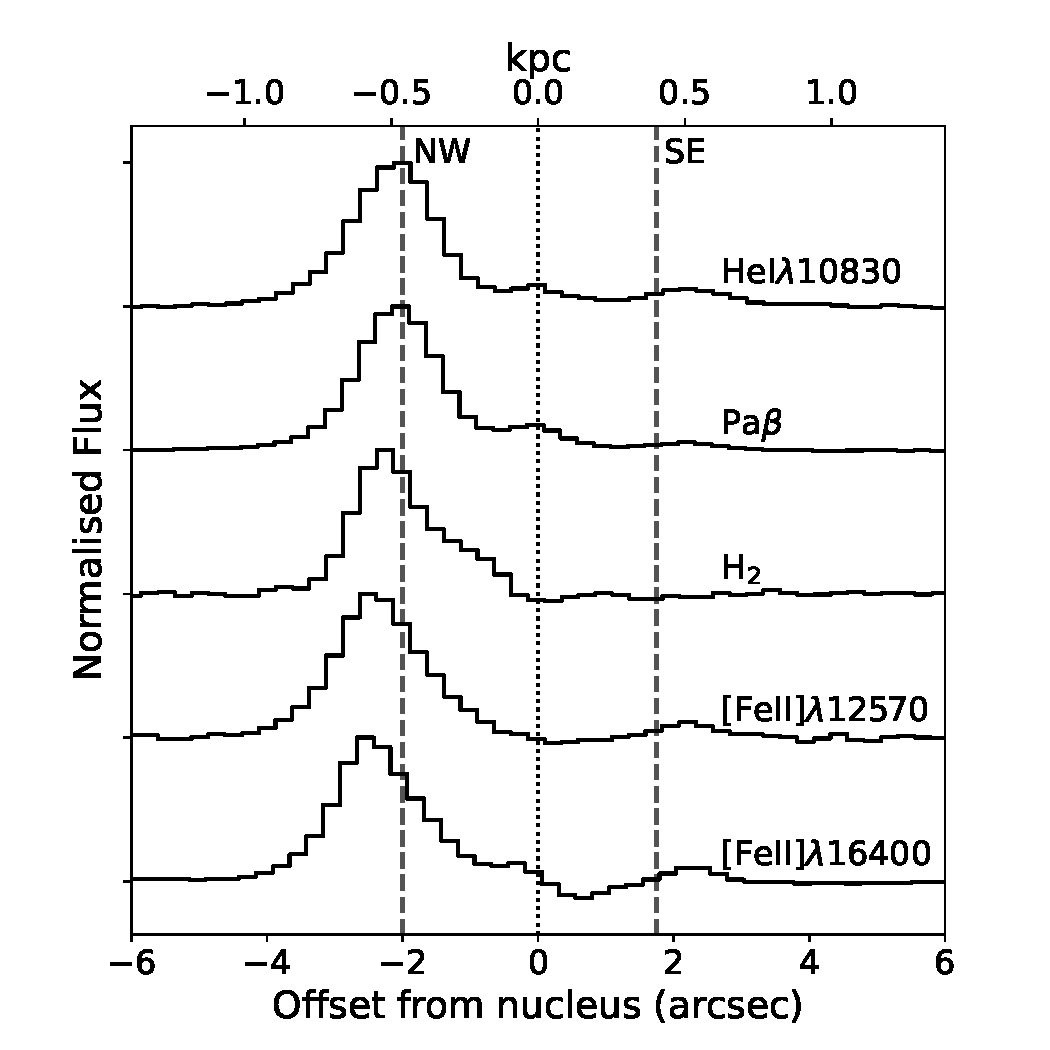
\includegraphics[width=0.7\linewidth]{figures/xshooter_ic5063/spatial_nir.pdf}
    \caption[Spatial flux distributions of the {[}FeII{]}$\lambda$16400, {[}FeII{]}$\lambda$12570, H$_\mathrm{2}\lambda$21218, Pa$\mathrm{\beta}$, and HeI$\lambda$10830 emission lines for the outflows in IC\;5063.]{Spatial flux distributions of the \mbox{$-$600\;\textless\;$v$ \;\textless\;$-$400\;km\;s$^{-1}$} wings of the emission-line profiles for [FeII]$\lambda$16400, [FeII]$\lambda$12570, H$_\mathrm{2}\lambda$21218, Pa$\mathrm{\beta}$, and HeI$\lambda$10830, produced using the same methodology as described in Section\;\ref{section: xshooter_ic5063: properties_of_outflowing_gas: uvb_vis_analysis_and_results: spatial_distributions}. It can be tentatively seen that the [FeII] lines (most likely tracing shocked warm-ionised emission) are emitted the furthest from the nucleus --- at the expected location of the shocks in the NW lobe --- with the warm-molecular H$_\mathrm{2}\lambda$21218 emission lying further inward, and the Pa$\mathrm{\beta}$ and HeI$\lambda$10830 emission lying closest to the nucleus. The centroids of Gaussian profiles fitted to these distributions are given in Table\;\ref{tab: xshooter_ic5063: spatial_nir}.}
    \label{fig: xshooter_ic5063: spatial_nir}
\end{figure}

\begin{table}[!t]
	\renewcommand{\arraystretch}{1.5}
    \centering
    \begin{tabular}{ccc}
    Emission Line           & Centroid (pixels) & Centroid (arcsec) \\ \hline
    HeI$\lambda$10830 & 8.5$\pm$0.2 & 2.11$\pm$0.05 \\
    Pa$\beta$ & 8.6$\pm$0.1 & 2.13$\pm$0.02 \\
    H$_\mathrm{2}\lambda$21218 & 9.5$\pm$0.1 & 2.36$\pm$0.02 \\
    {[FeII]$\lambda$12570} & 10.1$\pm$0.2 & 2.50$\pm$0.05 \\
    {[FeII]$\lambda$16400} & 10.2$\pm$0.2 & 2.53$\pm$0.05 \\                                                                                              
    \end{tabular}
    \caption[Measured centroids of Gaussian fits to the Spatial flux distributions of the {[}FeII{]}$\lambda$16400, {[}FeII{]}$\lambda$12570, H$_\mathrm{2}\lambda$21218, Pa$\mathrm{\beta}$, and HeI$\lambda$10830 emission lines for the outflows in IC\;5063.]{Centroids of Gaussian fits to spatial slices between \mbox{$-600$\;\textless\;$v$\;\textless\;$-400$\;km\;s$^{-1}$} of emission lines in the NIR arm data (Figure\;\ref{fig: xshooter_ic5063: spatial_nir}), measured relative to the spatial centroid position of the local continuum. The lines trace distinct phases of gas, which is interpreted here as a cooling sequence (Figure\;\ref{fig: xshooter_ic5063: cooling_sequence_schematic}).}
\label{tab: xshooter_ic5063: spatial_nir}
\end{table}

\subsubsection{Comparison to theoretical predictions of the dominant ionisation mechanism}
\label{section: xshooter_ic5063: discussion: mechanisms: model_comparison}

Relativistic hydrodynamic simulations by \citet{Meenakshi2022a} model the relative contribution of AGN-photoionisation and jet-induced-shock collisional-ionisation for a $5.71\times10^9$\;M$_\odot$ gas disk of radius 2\;kpc --- similar to the gas conditions and properties of IC\;5063 --- and find that shock-ionisation dominates the ionisation of the warm-ionised gas over AGN-photoionisation. This is inconsistent with the results presented here for IC\;5063, where AGN-photoionisation is found to be dominant. A potential reason for this discrepancy could be that the jet power in IC\;5063 is, in reality, an order of magnitude lower (P$_\mathrm{jet}$=10$^{44-45}$\;erg\;s$^{-1}$; \citealt{Mukherjee2018}) than assumed by \citet{Meenakshi2022a} (P$_\mathrm{jet}$=10$^{45}$\;erg\;s$^{-1}$). Moreover, the resolution of the simulations may not be sufficiently high to accurately track the density structure and cooling of the post-shock gas. Further simulation work that is more precisely tailored to the situation in IC\;5063 would allow this to be investigated in more detail, as would higher-resolution simulations of AGN and shock-ionisation for single clouds, which would allow a more accurate representation of the cooling of the warm gas.

\subsubsection{Compression effects of the jet-induced shocks}
\label{section: xshooter_ic5063: discussion: compression}

As the outflows along the radio-axis in IC\;5063 are likely to have been accelerated by jet-induced shocks, some evidence for shock-compression would be expected \citep{Sutherland2017}. Using the TR ratios (Section\;\ref{section: xshooter_ic5063: properties_of_outflowing_gas: uvb_vis_analysis_and_results: transauroral_lines}), it is found that the narrow components at all positions have relatively-low electron densities in the range \mbox{2.10\;\textless\;log$_{10}$(n$_e$[TR]\;cm$^{-3}$)\;\textless\;2.75}, while outflow components have significantly higher electron densities of \mbox{3.1\;\textless\;log$_{10}$(n$_e$[TR]\;cm$^{-3}$)\;\textless\;3.45}. This indicates that the outflows have higher electron densities than the quiescent gas by approximately a factor of three or four, possibly as a result of compression effects of the jet-induced shocks. This is similar to the findings of other AGN-driven-outflow studies, which find that broader components typically have higher densities \citep{Holt2011, Rose2018, Santoro2018, Santoro2020}, and is in line with what is expected for the immediate-post-shock gas due to the shock-jump conditions (a factor of four; \citealt{Sutherland2017}). However, the density contrast is much less than the factor of $\sim$100 which may be expected if the broad components originate from gas that has cooled in pressure equilibrium behind a fast shock \citep{Sutherland2017}.

\subsubsection{The nature of the blueshifted narrow [OIII] component seen in Aperture 3}
\label{section: xshooter_ic5063: discussion: ap3_narrow_component}

As seen in previous observations of the warm ionised phase of IC\;5063 \citep{Morganti2007}, a narrow kinematic component is identified at the position of the SE radio lobe that is blueshifted relative to the quiescent gas disk. Unlike the broad kinematic components associated with outflows, this component is narrow (\mbox{FWHM$_\mathrm{w}$\;\textless\;200\;km\;s$^{-1}$}) and has a lower electron density (log$_{10}n_\mathrm{e}=2.55\pm0.03$). Biconical outflows have been proposed to explain line splitting in active galaxies \citep{Walker1968, Cecil1990}, but if this is the case here, it is unclear why one direction of the outflow is broad and dense (AP3 Broad) and the other is narrow and has a lower density (AP3 Narrow 2). Alternatively, since IC\;5063 is thought to be a post-merger galaxy \citep{Morganti1998}, it would not be surprising to detect infalling and relatively-undisturbed low-density clumps of gas. Interestingly, H$_2$ emission that is kinematically associated with this component is not detected in Aperture\;3, implying that it either does not contain molecular gas or that the warm-molecular gas is not being excited. This is consistent with VLT/ISAAC observations presented by \citet{Tadhunter2014}, which show a blueshifted narrow component in the Br$\mathrm{\gamma}$ profile that is not present in the H$_2$1--0S(1) profile at the south-eastern lobe. Furthermore, this component is not seen in cold-molecular PV diagrams (e.g. CO(1--0), CO(2--1), CO(3--2), HCO(4--3); \citealt{Morganti2015, Oosterloo2017}), implying a lack of cold-molecular gas. Therefore, infalling gas is the favoured explanation, and I propose that the situation for Aperture 3 is as follows: the broad component represents shock-accelerated outflowing gas, the red-most narrow component represents quiescent gas in IC\;5063's disk, and the blue-most narrow component represents infalling gas (that lacks molecular-gas emission) as a result of the recent merger.

\vfill

\subsection{The use of transauroral-line diagnostics in AGN-driven outflows}
\label{section: xshooter_ic5063: discussion: transauroral_lines}

This study marks the first time that the transauroral-line technique first presented by \citet{Holt2011} has been used to estimate electron density values for spatially-resolved outflow regions in an active galaxy. As previously discussed, a concern with this technique is that the transauroral [OII] and [SII] lines might be emitted by different clouds at different spatial positions to those emitting other important diagnostic lines. The work presented here shows that the transauroral lines have the same line profiles for the same kinematic components and are emitted at the same spatial positions as the high-ionisation optical forbidden and recombination lines (Figures \ref{fig: xshooter_ic5063: o3_models_all_lines} and \ref{fig: xshooter_ic5063: spatial_optical}), suggesting that they are emitted by the same cloud complexes. While it is not conclusively demonstrated in this work that the transauroral lines are emitted by the same clouds \textit{within} the apertures (see discussions in \citealt{Sun2017} and \citealt{Rose2018}), this does alleviate concerns regarding their use in spatially-unresolved studies of moderate-to-high redshift AGN.

In addition, the transauroral-line technique has been used alongside the traditional [OII] and [SII] line ratios and [ArIV] line ratio to show that this method gives electron densities that are slightly higher than (if not comparable to) those given by the traditional line ratios, but lower than those given by the [ArIV] ratio. \citet{Wang2004} found that the [ArIV] technique provides much higher electron densities in observations of ionised nebulae than the traditional ratios; the findings presented here support this and place the transauroral-line technique in between these two methods in terms of derived densities. 

Further detailed studies making use of the transauroral-line ratios alongside other methods of electron-density estimation are needed. However, this work highlights the necessity of careful consideration of the technique used to derive electron densities: the traditional [OII] and [SII] lines may underestimate the electron density of warm-ionised outflowing gas, while the [ArIV] ratio may overestimate it. This, in part, may be due to the [ArIV] ratio probing higher-ionisation gas than the traditional and transauroral [OII] and [SII] techniques. Since the [OIII] lines represent higher-ionisation gas than the [OII] and [SII] lines, then the findings reported here indicate that the density of the [OIII]-emitting gas may be higher than probed by the [OII] and [SII] lines. It is unclear how this relates to the density of the H$\mathrm{\beta}$-emitting gas, although it could mean that true mass outflow rates (thus kinetic powers and coupling efficiencies) are even lower than estimated here, and much lower than typically derived using densities estimated with the traditional [SII] and [OII] ratios. A more detailed investigation of this situation is undertaken in Chapter\;\ref{chapter: stis_seyferts}.

The high electron densities (\mbox{$n_e$\;\textgreater\;10$^3$\;cm$^{-3}$}) found for the outflowing components using the TR ratios are above those typically assumed by past studies for warm-ionised outflows in active galaxies (\mbox{10$^{2}$--$10^3$\;cm$^{-3}$}: e.g. \citealt{Liu2013, Harrison2014, Fiore2017}), and are above the previously-measured maximum density of $n_e\sim10^3$\;cm$^{-3}$ for the warm-ionised gas along radio axis of IC\;5063, as derived from MUSE observations by \citet{Mingozzi2019} (see also \citealt{Venturi2021}). Conversely, the findings of this chapter support the results of other studies that report high electron densities for warm-ionised outflows, including those that also use transauroral lines (e.g. \citealt{Holt2011, Rose2018, Santoro2018, Spence2018, Baron2019b, Davies2020}). This highlights the importance of properly estimating values of electron density, and indicates that values determined solely using traditional techniques may be too low, and resulting kinetic powers too high.

Overall, these results show the validity of using the transauroral [SII] and [OII] lines in measuring the electron densities and reddening values of AGN-driven outflows: they have the advantages of higher critical densities (relative to the traditional [SII] and [OII] ratios), do not suffer from line blending issues, and are more prominent in galaxy spectra than the [ArIV] doublet.

\section{Chapter conclusions}
\label{section: xshooter_ic5063: conclusions}

Wide-wavelength-coverage, high spectral and spatial resolution Xshooter observations of the nearby active galaxy IC\;5063 have permitted, for the first time, electron density measurements of spatially-resolved AGN-driven outflows using the transauroral [SII] and [OII] lines. The wealth of previous observations of the different gas phases of these outflows has allowed the subsequently-derived warm-ionised outflow properties to be placed in a multi-phase context. In addition, the ionisation and excitation mechanisms of the outflows have been investigated for an object which shows clear jet-ISM interactions. This detailed study has found the following.
\begin{itemize}
    \item The transauroral lines are emitted in the same spatial positions and with the same line profiles as other high-ionisation optical lines which are commonly used for outflow diagnostics, indicating that they are emitted by the same cloud complexes. This alleviates concerns regarding the use of transauroral lines in spatially-unresolved studies of moderate-to-high redshift AGN.
    \item In the case of IC\;5063, there is tentative evidence that electron densities determined using the transauroral lines are higher than those determined from the commonly-used traditional [SII] and [OII] line ratios, and less than those produced using the higher-ionisation [ArIV](4711/4740) ratio. Given the implication for derived outflow kinetic powers if electron density is underestimated, this highlights that the transauroral lines should play an important role in future studies of AGN-driven outflows.
    \item The outflowing warm-ionised gas in IC\;5063 has a higher density than the quiescent gas, potentially as a result of compression effects of jet-induced shocks. However, the outflow densities may be below those expected if the post-shock gas is cooling in pressure equilibrium.
    \item The kinetic powers for the warm ionised phase are much below those required by galaxy evolution models. However, when compared to previous observations of cooler phases, it appears that this phase constitutes only a small fraction of the total outflowing mass; the neutral atomic phase dominates the mass and kinetic power of the \textit{total} outflow.
    \item The dominant ionisation mechanism of the warm-ionised outflows and quiescent gas is AGN-photoionisation, while the warm-molecular outflows appear to be excited by composite AGN-shock excitation. A possible scenario is that the post-shock gas closest to the AGN is maintained in an ionised state by photoionisation, and forms the ionised part of an ISM component that shields the immediate-post-shock gas that lies further from the AGN, allowing it to cool to colder phases.
\end{itemize}

\section*{Chapter acknowledgements}
\label{section: xshooter_ic5063: acknowledgements}
\addcontentsline{toc}{section}{\protect\numberline{}Chapter acknowledgements}

Based on observations collected at the European Organisation for Astronomical Research in the Southern Hemisphere under ESO programme 0101.B0409(A). This work makes use of the Starlink software \citep{Currie2014}, which is currently supported by the East Asian Observatory. This research has made use of the NASA/IPAC Infrared Science Archive, which is funded by the National Aeronautics and Space Administration and operated by the California Institute of Technology. The STARLIGHT project is supported by the Brazilian agencies CNPq, CAPES and FAPESP and by the France-Brazil CAPES/Cofecub program. I thank Rebecca J. Houghton for her helpful comments in preparing this manuscript, and Moun Meenakshi and Dipanjan Mukherjee for their useful discussion.

\section*{Data availability}
\addcontentsline{toc}{section}{\protect\numberline{}Data availability}

The data used in this chapter is available from the ESO Science Archive Facility (\url{http://archive.eso.org/cms.html}) with Run/Program ID 0101.B-0409(A) (PI: Tadhunter).
